% slurmcmc -- theory and user manual
% Build:  latexmk -lualatex theory_and_manual.tex   (LuaLaTeX, for the shaded inline code; figures from ../pics)
\documentclass[11pt,a4paper,openany]{report}

% ---------------------------------------------------------------- typography
\usepackage[T1]{fontenc}
\usepackage{newpxtext,newpxmath}
\usepackage[scaled=0.86]{beramono}
\usepackage{microtype}
\usepackage[a4paper,margin=2.6cm,headheight=14pt]{geometry}
\linespread{1.05}
\setlength{\parskip}{0.45em}
\setlength{\parindent}{0pt}
\setlength{\emergencystretch}{2.5em}   % loosen a line rather than overrun the margin

% ---------------------------------------------------------------- mathematics
\usepackage{amsmath,amssymb,bm}
\newcommand{\pexp}{p_{\mathrm{exp}}}
\newcommand{\psur}{p_{\mathrm{sur}}}
\newcommand{\ESS}{\mathrm{ESS}}
\newcommand{\ESSw}{\mathrm{ESS}_w}
\newcommand{\Lc}{L_c}
\newcommand{\Nc}{N_c}
\newcommand{\R}{\mathbb{R}}

% ---------------------------------------------------------------- colour and boxes
\usepackage{xcolor}
\definecolor{accent}{RGB}{31,78,121}
\definecolor{accentsoft}{RGB}{232,239,246}
\definecolor{caution}{RGB}{166,97,0}
\definecolor{codebg}{RGB}{247,248,250}
\definecolor{inlinecodebg}{RGB}{232,235,239}
\usepackage[most]{tcolorbox}
\newtcolorbox{keypoint}[1][Key point]{enhanced, breakable, colback=accentsoft, colframe=accent,
  boxrule=0pt, leftrule=3pt, arc=0pt, outer arc=0pt, left=9pt, right=9pt, top=6pt, bottom=6pt,
  fonttitle=\bfseries\small, coltitle=accent, colbacktitle=accentsoft, titlerule=0pt,
  title={#1}, before skip=10pt, after skip=10pt}
\newtcolorbox{cautionbox}[1][Caution]{enhanced, breakable, colback=caution!6, colframe=caution,
  boxrule=0pt, leftrule=3pt, arc=0pt, outer arc=0pt, left=9pt, right=9pt, top=6pt, bottom=6pt,
  fonttitle=\bfseries\small, coltitle=caution, colbacktitle=caution!6, titlerule=0pt,
  title={#1}, before skip=10pt, after skip=10pt}

% ---------------------------------------------------------------- code
\usepackage{listings}
\lstdefinestyle{py}{language=Python, basicstyle=\ttfamily\small, keywordstyle=\color{accent}\bfseries,
  commentstyle=\color{black!50}\itshape, stringstyle=\color{teal!65!black},
  backgroundcolor=\color{codebg}, frame=l, framerule=2pt, rulecolor=\color{accent!35},
  framesep=8pt, xleftmargin=10pt, aboveskip=8pt, belowskip=8pt, showstringspaces=false,
  columns=fullflexible, keepspaces=true, breaklines=true, upquote=true}
\lstdefinestyle{plain}{style=py, language={}, keywordstyle={}, stringstyle={}}
\lstset{style=py}
% inline code on a grey background, as on GitHub; lua-ul keeps the shading across the line
% breaks allowed after _ . / , ( so long identifiers never overrun the margin
\usepackage{luacolor,lua-ul}
\usepackage[obeyspaces]{url}
\DeclareUrlCommand\codeinner{\urlstyle{tt}\def\UrlBreaks{\do\_\do\.\do\/\do\,\do\(}}
\newcommand{\code}[1]{\leavevmode\highLight[inlinecodebg]{\kern1.5pt\codeinner{#1}\kern1.5pt}}

% ---------------------------------------------------------------- tables and figures
\usepackage{booktabs,tabularx,xltabular,array}
\newcolumntype{L}{>{\raggedright\arraybackslash}X}
\renewcommand{\arraystretch}{1.2}
\usepackage{graphicx}
\graphicspath{{../pics/}}
\usepackage{float}
\usepackage{needspace}
\usepackage[font=small,labelfont={bf,color=accent},skip=6pt,margin=0.5cm]{caption}
% argument reference tables: name, default, meaning
\newenvironment{argtable}
  {\footnotesize\setlength{\tabcolsep}{5pt}\renewcommand{\arraystretch}{1.2}%
   \xltabular{\linewidth}{@{}>{\raggedright\arraybackslash}p{0.30\linewidth}%
   >{\raggedright\arraybackslash}p{0.13\linewidth}L@{}}
   \toprule \textbf{argument} & \textbf{default} & \textbf{meaning}\\ \midrule \endhead
   \bottomrule \endfoot}
  {\endxltabular}

% ---------------------------------------------------------------- headings and page style
\usepackage{titlesec}
\titleformat{\chapter}[display]{\normalfont\color{accent}\raggedright}
  {\large\scshape \chaptertitlename~\thechapter}{2pt}{\huge\bfseries}[\vspace{4pt}{\titlerule[1pt]}]
\titlespacing*{\chapter}{0pt}{-12pt}{22pt}
\titleformat{\section}{\normalfont\Large\bfseries\color{accent}}{\thesection}{0.8em}{}
\titleformat{\subsection}{\normalfont\large\bfseries}{\thesubsection}{0.8em}{}
\titleformat{\subsubsection}{\normalfont\normalsize\bfseries\itshape}{}{0em}{}
\titlespacing*{\section}{0pt}{16pt}{6pt}
\titlespacing*{\subsection}{0pt}{12pt}{4pt}
\usepackage{fancyhdr}
\pagestyle{fancy}
\fancyhf{}
\fancyhead[L]{\small\color{black!55}\nouppercase{\leftmark}}
\fancyhead[R]{\small\color{black!55}\textsf{slurmcmc}}
\fancyfoot[C]{\small\thepage}
\renewcommand{\headrulewidth}{0.3pt}
\renewcommand{\chaptermark}[1]{\markboth{\thechapter.\ #1}{}}
\fancypagestyle{plain}{\fancyhf{}\fancyfoot[C]{\small\thepage}\renewcommand{\headrulewidth}{0pt}}

\usepackage{enumitem}
\setlist{itemsep=2pt, topsep=4pt}
\usepackage[colorlinks=true, linkcolor=accent, urlcolor=accent, citecolor=accent,
            pdftitle={slurmcmc: theory and user manual}]{hyperref}
\usepackage[capitalise,noabbrev]{cleveref}

\begin{document}

% ---------------------------------------------------------------- title page
\begin{titlepage}
  \centering
  \vspace*{1.5cm}
  
\includegraphics[width=0.95\textwidth]{logo.jpeg}\par
  \vspace{1.6cm}
  {\color{accent}\rule{0.95\textwidth}{1pt}}\par\vspace{0.6cm}
  {\fontsize{34}{40}\selectfont\bfseries\color{accent} slurmcmc\par}
  \vspace{0.35cm}
  {\LARGE Theory and User Manual\par}
  \vspace{0.6cm}
  {\color{accent}\rule{0.95\textwidth}{1pt}}\par
  \vspace{1.2cm}
  {\large Bayesian model calibration of expensive black-box models\\
   with parallel optimization, ensemble MCMC and surrogate models\\
   on a Slurm cluster\par}
  \vfill
  {\large Version 2.0\par}
  \vspace{0.3cm}
  {\large \today\par}
\end{titlepage}

\pagenumbering{roman}
\tableofcontents
\clearpage
\pagenumbering{arabic}

\chapter{Introduction}
\label{ch:intro}

\section{Bayesian model calibration}

A physical model predicts observations $y$ from a vector of parameters $\theta \in \R^d$.
\emph{Calibrating} the model means answering two questions: which parameters make it agree with
the data, and how well the data actually pin those parameters down. Bayesian model calibration
answers both at once, with the posterior distribution
\begin{equation}
  p(\theta \mid y) \;\propto\; \mathcal{L}(y \mid \theta)\,\pi(\theta),
  \label{eq:bayes}
\end{equation}
the likelihood of the data under the model, times a prior. In practice one works with its
logarithm,
\begin{equation}
  \log p(\theta) \;=\; \log \mathcal{L}(y \mid \theta) + \log \pi(\theta) + \text{const},
  \label{eq:logpost}
\end{equation}
which is only ever known up to that additive constant. The constant does not matter: the
posterior is unchanged by $\log p \to \log p + c$, and every algorithm in this manual is built so
that it never needs it.

The obstacle is cost. Each evaluation of $\log p$ runs the forward model --- a simulation that can
take minutes or hours --- and the algorithms that explore a posterior need thousands to millions of
evaluations. \textbf{slurmcmc} makes this tractable on a Slurm cluster in three ways: it evaluates
as many parameter points \emph{simultaneously} as an algorithm allows; it keeps a complete,
restartable record of every evaluation, so no expensive work is ever repeated; and, when even that
is not enough, it replaces most evaluations with a fast surrogate model while measuring whether the
surrogate can be trusted.

\section{The workflow}

A calibration typically goes through three stages, which is also how this manual is organised.

\begin{enumerate}[leftmargin=*, label=\textbf{\arabic*.}]
  \item \textbf{Optimization} (\cref{ch:optimization}). Minimize a loss that measures the misfit
        to data. This checks that the model \emph{can} represent the data at all, before any
        effort is spent on uncertainty, and it finds the region where the posterior lives, which
        is where MCMC should start.
  \item \textbf{MCMC} (\cref{ch:mcmc}). Sample the posterior with an ensemble Markov chain Monte
        Carlo algorithm whose walkers are evaluated in parallel on the cluster.
  \item \textbf{Surrogate-based MCMC} (\cref{ch:surrogate,ch:hybrid}). When a full MCMC is
        unaffordable, fit a fast surrogate to a limited number of expensive evaluations and sample
        the surrogate instead. The automated \emph{hybrid} pipeline iterates this until measured
        criteria say the surrogate posterior can be trusted.
\end{enumerate}

All three share the same machinery for dispatching evaluations to the cluster, recording them,
and restarting interrupted runs. \Cref{ch:parallel} describes it once, so the later chapters can
concentrate on the algorithms.

\section{What the package is built on}

slurmcmc stitches together established libraries rather than re-implementing them:

\begin{center}
\small
\begin{tabularx}{\linewidth}{@{}l L@{}}
  \toprule
  \textbf{library} & \textbf{role in slurmcmc} \\
  \midrule
  \href{https://github.com/facebookincubator/submitit}{\texttt{submitit}} &
    submits evaluations as Slurm job arrays (or local processes) and collects their results \\
  \href{https://github.com/facebookresearch/nevergrad}{\texttt{nevergrad}} &
    gradient-free population optimizers: Differential Evolution, Particle Swarm, and others \\
  \href{https://github.com/pytorch/botorch}{\texttt{botorch}} &
    Bayesian optimization with a Gaussian-process model \\
  \href{https://github.com/dfm/emcee}{\texttt{emcee}} &
    the affine-invariant ensemble MCMC sampler \\
  \href{https://scikit-learn.org}{\texttt{scikit-learn}} &
    the Gaussian-process and polynomial surrogate models of the hybrid pipeline \\
  \bottomrule
\end{tabularx}
\end{center}

and exposes four entry points:

\begin{center}
\small
\begin{tabularx}{\linewidth}{@{}l l L@{}}
  \toprule
  \textbf{entry point} & \textbf{module} & \textbf{purpose} \\
  \midrule
  \code{slurm_minimize}    & \code{slurmcmc.optimization} & parallel minimization of a loss (\cref{ch:optimization}) \\
  \code{slurm_mcmc}        & \code{slurmcmc.mcmc}         & ensemble MCMC with walkers evaluated on the cluster (\cref{ch:mcmc}) \\
  \code{slurm_mcmc_hybrid} & \code{slurmcmc.hybrid}       & automated surrogate-based MCMC (\cref{ch:hybrid}) \\
  \code{SlurmPool}         & \code{slurmcmc.slurm_utils}  & a cluster-backed \code{map}, used by all of the above and usable on its own (\cref{ch:parallel}) \\
  \bottomrule
\end{tabularx}
\end{center}

\section{Installation}

Install the package from the repository root; its core dependencies are pulled in automatically:
\begin{lstlisting}[style=plain]
pip install -e .
\end{lstlisting}
Bayesian optimization needs the \code{botorch} extra and the hybrid pipeline the \code{hybrid}
extra (scikit-learn). The \code{examples} and \code{test} extras add what the example scripts and
the test suite need. To install everything at once:
\begin{lstlisting}[style=plain]
pip install -e ".[botorch,hybrid,examples,test]"
\end{lstlisting}
Python~3.10 or newer is required. On a shared cluster without administrator rights, add
\code{--user} to install into your home directory.

\section{Running the tests}

\begin{lstlisting}[style=plain]
pytest -vv tests
\end{lstlisting}
Tests that need a real Slurm cluster are skipped automatically elsewhere; a mock-Slurm test file
exercises the Slurm code path without one.

\section{The examples behind this manual}

Every figure in this manual is produced by one of the example scripts in the \code{examples}
directory, so every result shown can be reproduced, and each script doubles as a starting point for
a real problem.

\begin{center}
\small
\begin{tabularx}{\linewidth}{@{}l L@{}}
  \toprule
  \textbf{script} & \textbf{shown in} \\
  \midrule
  \code{example_optimization.py}                   & \cref{sec:opt-example} \\
  \code{example_optimization_algorithms_comparison.py} & \cref{sec:opt-comparison} \\
  \code{example_mcmc.py}                           & \cref{sec:mcmc-example} \\
  \code{example_mcmc_and_mc_comparison.py}         & \cref{sec:mcmc-vs-mc} \\
  \code{example_mcmc_surrogate.py}                 & \cref{sec:surrogate-example} \\
  \code{example_mcmc_hybrid.py}                    & \cref{sec:hybrid-example} \\
  \bottomrule
\end{tabularx}
\end{center}

\chapter{Evaluating an expensive function in parallel}
\label{ch:parallel}

Every algorithm in the package needs the same service: evaluate a function at a batch of points,
as many at once as the cluster allows, and never lose or repeat an evaluation. This chapter
describes that shared layer. The arguments introduced here behave identically in
\code{slurm_minimize}, \code{slurm_mcmc} and \code{slurm_mcmc_hybrid}; \cref{app:common} collects
them in one table.

\section{The function you supply}

The expensive function takes a parameter vector --- a NumPy array of length $d$ --- and returns a
single number: a loss to be minimized (\cref{ch:optimization}), or a log-probability to be sampled
(\cref{ch:mcmc,ch:surrogate,ch:hybrid}), known up to a constant.

\begin{lstlisting}
def log_prob(theta):
    write_simulation_input(theta)      # e.g. a namelist for the forward code
    run_simulation()                   # minutes to hours
    return -0.5 * chi_squared(read_simulation_output())
\end{lstlisting}

Three facilities make real forward models easy to plug in.

\textbf{Its own working directory.} On the cluster each evaluation runs with its current directory
set to a directory of its own (\cref{sec:audit}), so the function can write input files, launch an
external code and parse its output without evaluations interfering with each other --- and every
file it writes stays behind as a record.

\textbf{A constant extra argument.} Anything the function needs besides $\theta$ --- the data, a
configuration dictionary, a path --- can be passed once as \code{extra_arg}. The function is then
called as \code{fun(theta, extra_arg)}.

\textbf{Deferred import.} A function has to be pickled to be sent to a compute node, and functions
defined in a script or notebook often cannot be. Instead of the function, pass where to find it:
\begin{lstlisting}
log_prob_fun = {'module_dir': '/home/me/model',
                'module_name': 'my_model',
                'function_name': 'log_prob'}
\end{lstlisting}
Only the three names are pickled. The function is imported inside each job, and re-imported fresh
there, so edits to the module are picked up by later evaluations. The same form is accepted for
\code{constraint_fun}.

\section{SlurmPool: one job array per batch}
\label{sec:slurmpool}

\code{SlurmPool} provides a single method, \code{map(fun, points)}, that returns the function's
value at each point, in order. It is a drop-in replacement for the \code{map} of
\code{multiprocessing.Pool} --- which is exactly how \code{emcee} uses it to evaluate its walkers.

Each call to \code{map} is submitted as \textbf{one Slurm job array}, named
\code{<job_name>_<call number>}, whose task $k$ evaluates point $k$. An iteration of an optimizer or
of MCMC is therefore a single scheduler transaction, however many points it contains. Batches larger
than \code{budget} points are split into consecutive arrays of at most that size.

\code{SlurmPool} can also be used on its own, for instance for a parameter scan:
\begin{lstlisting}
from slurmcmc.slurm_utils import SlurmPool

pool = SlurmPool(work_dir='scan', job_name='scan', cluster='slurm',
                 dim_input=3, dim_output=1,
                 submitit_kwargs={'slurm_partition': 'compute', 'timeout_min': 60})
values = pool.map(log_prob, points)
\end{lstlisting}

\section{Where the evaluations run}

The \code{cluster} argument selects the execution backend:

\begin{center}
\small
\begin{tabularx}{\linewidth}{@{}l L@{}}
  \toprule
  \code{cluster} & \textbf{behaviour} \\
  \midrule
  \code{'slurm'}     & submit job arrays to a Slurm cluster through submitit \\
  \code{'local'}     & run as local processes through submitit's local executor, with the same
                       directory layout as \code{'slurm'} --- useful for debugging the file handling \\
  \code{'local-map'} & evaluate sequentially inside the calling process: no jobs and no
                       directories. Fastest for cheap analytic functions and for tests \\
  \bottomrule
\end{tabularx}
\end{center}

A practical progression is to develop with \code{'local-map'}, check the files a real evaluation
writes with \code{'local'}, and then run with \code{'slurm'}. Scheduler options --- partition, time
limit, cores, memory --- are passed through \code{submitit_kwargs}, which is forwarded to submitit's
\code{AutoExecutor.update_parameters} (for example \code{slurm_partition}, \code{timeout_min},
\code{cpus_per_task}, \code{mem_gb}).

\section{The audit trail}
\label{sec:audit}

With \code{'slurm'} or \code{'local'}, every evaluation leaves a directory behind:

\begin{lstlisting}[style=plain]
work_dir/
  points_history.txt      every point of every call, led by call and point index
  values_history.txt     the corresponding results
  0/                  the first map() call, e.g. iteration 0
    inputs.txt        every point of the call, one per row
    outputs.txt       the corresponding results
    extra_arg.pkl     the extra_arg, when one was given
    0/
      input.txt       the point
      output.txt      its result
      ...             anything the function itself wrote
    1/
    ...
  1/                  the second call
  ...
\end{lstlisting}

The submitit logs of each job sit in the call's directory too, so a failed evaluation can be
debugged from its own inputs, outputs and error log, and a point's own output files can be re-used
later, for instance to compute a different quantity from the same runs. Once a call's results are
in, its points and results are also appended to \code{work_dir/points_history.txt} and
\code{work_dir/values_history.txt}, one row per point, led by the call and point indices.

When only the results matter, the call directories are clutter. \code{keep_run_dirs} decides what
stays: \code{'all'} (the default) keeps them, \code{'failed'} removes those in which every
evaluation succeeded, and \code{'none'} removes them all. The two history files are written in
every mode. A fresh run expects \code{work_dir} not to hold an earlier run's output, numbered call
directories or \code{points_history.txt}; use a new \code{work_dir}, or resume the old run from its
restart file (\cref{sec:restart}).

\section{Failures}
\label{sec:failures}

On a cluster some evaluations fail: a node dies, a simulation diverges, a job runs out of time.
An evaluation is counted as \textbf{failed} when
\begin{itemize}
  \item it returns \code{None}, NaN, or \code{job_fail_value};
  \item its job raises an exception; or
  \item it stays in the running state longer than \code{check_output_timeout_minutes}, in which case
        its job is cancelled.
\end{itemize}
Its result is then recorded as \code{job_fail_value}, and the run continues. The default is NaN for
minimization and $-10^{10}$ for the MCMC functions: a walker proposed into a failed point sees an
extremely low log-probability and simply rejects the move. Failed \emph{submissions} --- a
scheduler hiccup rather than a failed evaluation --- are retried up to
\code{submit_retry_max_attempts} times, \code{submit_retry_wait_seconds} apart;
\code{submit_delay_seconds} adds a pause after each submission, and
\code{check_output_interval_seconds} sets how often job states are polled.

\section{The evaluation history}

Every point a pool has evaluated is recorded. The pool, returned in each function's status as
\code{status['slurm_pool']}, exposes:

\begin{center}
\small
\begin{tabularx}{\linewidth}{@{}l L@{}}
  \toprule
  \textbf{attribute} & \textbf{content} \\
  \midrule
  \code{points_history}       & all evaluated points, in submission order, shape $(n, d)$ \\
  \code{values_history}       & their results, shape $(n, 1)$; failed points hold \code{job_fail_value} \\
  \code{inds_success_points}, \code{inds_failed_points} & row indices of successful and failed evaluations \\
  \code{evaluated_points_set} & the set of evaluated points, for instant duplicate checks \\
  \code{point_loc_dict}       & for each point, the (call, index) directory holding its files \\
  \code{num_evaluated_points} & the total count \\
  \bottomrule
\end{tabularx}
\end{center}

The duplicate check is what lets \code{slurm_minimize} guarantee it never pays twice for the same
point, and the history is what a surrogate is trained on. For very long MCMC runs whose history is
not needed, \code{record_history=False} saves the memory --- and time, since the bookkeeping grows
with the number of evaluations. It governs these in-memory arrays only: the same record is written
to disk as it goes, in \code{points_history.txt} and \code{values_history.txt} (\cref{sec:audit}).

\section{Restarting an interrupted run}
\label{sec:restart}

A calibration can run for days, and jobs get killed. With \code{save_restart=True} the complete
state of a run --- optimizer or sampler, evaluation history, iteration counter --- is written to
\code{work_dir/restart_file} after every \code{restart_save_interval} iterations. The write is
atomic: the file is written under a temporary name and then renamed, so a job killed mid-save
leaves the previous restart file intact.

A \code{SlurmPool} used on its own has no restart file of its own; it takes \code{load_restart=True}
instead, which rebuilds its call counter and its history from the two history files and continues
the numbering, evaluating whatever the next \code{map()} is given.

To continue, call the same function again with \code{load_restart=True}. It resumes from the saved
state and runs \code{num_iters} \emph{further} iterations, so the same call also extends a run that
finished. The default file names are \code{opt_restart.pkl}, \code{mcmc_restart.pkl} and
\code{hybrid_restart.pkl}; \code{slurm_mcmc} and \code{slurm_mcmc_hybrid} also accept the state as
an in-memory dictionary, \code{status_restart}.

By default each function installs a handler for \code{SIGTERM}, so that a run cancelled with
\code{scancel} exits with an error code and Slurm marks it as failed rather than completed. Pass
\code{install_signal_handler=False} when embedding a run in an application that manages its own
signals.

\section{Reproducible runs}
\label{sec:seed}

Every algorithm in the package makes random choices: the proposals of an MCMC sampler, the
candidates of an optimizer, the validation points and model fits of the hybrid pipeline. Pass
\code{random_seed} to make a run reproducible:
\begin{lstlisting}
status = slurm_mcmc(..., random_seed=0)
\end{lstlisting}
The seed is applied at the start of the loop, inside the process that runs it --- not by the
script that calls the function. That distinction matters in remote mode (\cref{sec:remote}): the
loop then runs in a fresh process on a compute node, which a \code{np.random.seed} call in the
submitting script never reaches, so without \code{random_seed} a remote run follows a different
trajectory from the same configuration. It seeds numpy's global generator, from which \texttt{emcee},
\texttt{nevergrad} and scikit-learn draw, Python's own generator, and torch's when \texttt{botorch}
is in use.

The restart file stores the state of those generators, so a run that was interrupted and resumed
reproduces the run that was never interrupted, iteration for iteration.

\begin{cautionbox}[Reproducible on the same software stack]
A seed fixes every random choice, not the arithmetic. Different versions of numpy, scipy or
scikit-learn, or a different linear-algebra library or CPU, change results in the last digits, and a
long MCMC or a sequence of model fits amplifies those differences. Expect identical results from the
same environment, and statistically equivalent ones elsewhere. A function that is itself random, such
as a stochastic simulation, has to seed itself.
\end{cautionbox}

\section{Running the whole loop as a job: remote mode}
\label{sec:remote}

The loop that drives an optimization or MCMC --- asking for points, waiting for their jobs,
updating the algorithm --- is itself a long-running process. Login nodes usually limit how long a
process may run. With \code{remote=True} the whole loop is instead submitted as a job of its own:
its configuration is pickled and run on \code{remote_cluster} (\code{'slurm'} or \code{'local'}),
under the name \code{main_{job_name}}, with a 30-day time limit unless
\code{remote_submitit_kwargs} says otherwise.

The call then returns a submitit \code{Job} immediately, instead of the status dictionary.
\code{job.result()} waits for the run to finish and returns the same dictionary a local run would.
submitit also stores it in \code{work_dir} as \code{<job_id>_0_result.pkl}, so it can be recovered
later from nothing but the directory and the job id:
\begin{lstlisting}
import submitit
status = submitit.SlurmJob(folder='mcmc', job_id='123456').result()
\end{lstlisting}

\begin{keypoint}[What survives a remote run]
The result file is written only when the job finishes. A failed job stores its traceback there
instead, and \code{.result()} raises it; a job killed before the end leaves no result file at all,
but its restart file (\cref{sec:restart}) is still there to resume from.
\end{keypoint}

\section{Configuration objects}

Each entry point is a thin wrapper that packs its keyword arguments into a configuration dataclass
and runs it. The dataclasses and runners can be used directly, for instance to build, inspect or
store a configuration before running it:
\begin{lstlisting}
from slurmcmc.optimization import MinimizeConfig, Minimizer
from slurmcmc.mcmc import MCMCConfig, MCMCRunner
from slurmcmc.hybrid import HybridMCMCConfig, HybridMCMCRunner

status = MCMCRunner(MCMCConfig(log_prob_fun=log_prob, init_points=init_points,
                               num_iters=1000)).run()
\end{lstlisting}

\chapter{Optimization}
\label{ch:optimization}

\section{Why optimize first}

Before asking how uncertain the parameters are, it is worth asking whether the model can represent
the data at all. Optimization answers that: minimize a loss $f(\theta)$ that measures the misfit,
for example $\chi^2(\theta)$, and check that its minimum is statistically acceptable. If it is not,
no amount of posterior sampling will help --- the problem lies with the model. If it is, the
minimizer has also located the region where the posterior lives, which is exactly where MCMC should
start its walkers (\cref{ch:mcmc}).

The problem solved is a bounded, optionally constrained minimization,
\begin{equation}
  \min_{\theta}\; f(\theta)
  \quad\text{subject to}\quad
  \theta \in [\ell_1, u_1] \times \dots \times [\ell_d, u_d],
  \qquad c(\theta) \le 0,
  \label{eq:minimize}
\end{equation}
where the box is \code{param_bounds} and $c$ is the optional \code{constraint_fun}: a point is
feasible when $c(\theta) \le 0$. The function $f$ is a black box: no gradients, and every value
costs an expensive evaluation. What can be parallelized is the number of points evaluated per
iteration, \code{num_workers}.

\section{The algorithms}

Three families are available. The first two are population methods from \texttt{nevergrad}; the
third builds a statistical model of $f$.

\subsection{Differential Evolution (default)}

Differential Evolution (DE) keeps a population of candidate points and improves it generation by
generation. For each member $\theta_i$ it builds a mutant from three other members,
\begin{equation}
  v_i = \theta_a + F\,(\theta_b - \theta_c),
\end{equation}
mixes coordinates of the mutant and of $\theta_i$ (crossover) into a trial point, and replaces
$\theta_i$ by the trial point if it has a lower loss. The difference vectors adapt the step size
to the population's own spread, which makes DE robust on rugged and badly scaled losses. The
default in slurmcmc is \texttt{nevergrad}'s DE with two-point crossover and a population equal to
\code{num_workers}, so one generation is exactly one iteration of parallel evaluations.

\subsection{Particle Swarm Optimization}

Particle Swarm Optimization (PSO) moves each particle with a velocity that is pulled towards the
best point the particle has seen, $p_i$, and the best point the swarm has seen, $g$:
\begin{equation}
  u_i \leftarrow \omega\, u_i + c_1 r_1 (p_i - \theta_i) + c_2 r_2 (g - \theta_i),
  \qquad
  \theta_i \leftarrow \theta_i + u_i,
\end{equation}
where $r_1$ and $r_2$ are random numbers in $[0,1]$. Select it with
\code{optimizer_class=ng.optimizers.ConfPSO(popsize=num_workers)}; any other \texttt{nevergrad}
optimizer can be passed the same way.

\subsection{Bayesian optimization}

Bayesian optimization (BO), with \code{optimizer_package='botorch'}, fits a Gaussian-process model
to all evaluations so far and uses it to decide where to evaluate next. The model gives, at every
point, a predicted loss and an uncertainty. A candidate is chosen to maximize the expected
improvement over the best loss found so far, $f^\ast$,
\begin{equation}
  \mathrm{EI}(\theta) \;=\; \mathbb{E}\!\left[\max\!\big(f^\ast - f(\theta),\, 0\big)\right],
\end{equation}
which balances exploiting regions of low predicted loss against exploring regions of high
uncertainty. slurmcmc uses \texttt{botorch}'s batch version, \code{qLogExpectedImprovement}, to
propose \code{num_workers} points per iteration, with inputs normalized and outputs standardized;
the first iteration, with no data yet, uses a quasi-random Sobol design.

BO spends far fewer evaluations when each one is very expensive, but the model has a cost of its
own. Fitting a Gaussian process to $n$ points scales as $\mathcal{O}(n^3)$, and it is refitted every
iteration, so a long run slows down. Two options in \code{botorch_kwargs} address this:

\begin{center}
\small
\begin{tabularx}{\linewidth}{@{}l l L@{}}
  \toprule
  \textbf{key} & \textbf{default} & \textbf{meaning} \\
  \midrule
  \code{num_best_points} & \code{None} & train the model only on this many lowest-loss points, keeping each fit bounded in size \\
  \code{sequential}      & \code{True} & choose the batch greedily, one point at a time, rather than optimizing all $q\times d$ coordinates jointly; much faster at equivalent quality \\
  \code{num_restarts}    & \code{10}   & restarts of the acquisition-function optimization \\
  \code{raw_samples}     & \code{100}  & random samples seeding those restarts \\
  \code{options}         & \code{None} & extra options for \texttt{botorch}'s \code{optimize_acqf} \\
  \bottomrule
\end{tabularx}
\end{center}

\section{How a batch of candidates is chosen}

Each iteration, \code{slurm_minimize} asks the optimizer for candidates until it holds
\code{num_workers} of them that are
\begin{itemize}
  \item \textbf{new} --- not evaluated in any earlier iteration, nor already in this batch;
  \item \textbf{feasible} --- satisfying \code{constraint_fun} $\le 0$, which is evaluated cheaply
        before any expensive job is spent on the point.
\end{itemize}
Only then is the batch submitted as one job array. If \code{num_asks_max} requests pass without
completing the batch --- typically because the feasible region is tiny --- the run stops with an
error rather than looping forever.

Starting points can be supplied as \code{init_points}; they are evaluated in the first iteration
and must satisfy the constraint. An iteration in which \emph{every} evaluation failed stops the
run, since the optimizer would have nothing to learn from.

\needspace{14\baselineskip}
\section{Usage}

\begin{lstlisting}
import numpy as np
from slurmcmc.optimization import slurm_minimize

def loss_fun(x):
    return (1 - x[0])**2 + 100 * (x[1] - x[0]**2)**2

def constraint_fun(x):                      # feasible when <= 0
    return (x[0] + 1)**2 + (x[1] + 1)**2 - 16

status = slurm_minimize(loss_fun=loss_fun, constraint_fun=constraint_fun,
                        param_bounds=[[-5, 5], [-5, 5]],
                        num_workers=10, num_iters=30,
                        cluster='slurm', work_dir='minimize', save_restart=True)
print(status['x_min'], status['loss_min'])
\end{lstlisting}

The arguments specific to minimization are listed below; those shared by every function are in
\cref{app:common}.

\begin{argtable}
  \code{loss_fun} & required & the loss, \code{f(x)} or \code{f(x, extra_arg)}; a callable or a deferred-import dictionary \\
  \code{param_bounds} & required & \code{[[lo, hi], ...]}, one pair per parameter \\
  \code{num_workers} & required & points evaluated in parallel per iteration \\
  \code{num_iters} & required & iterations to run (further iterations, when resuming) \\
  \code{optimizer_package} & \code{'nevergrad'} & \code{'nevergrad'} or \code{'botorch'} \\
  \code{optimizer_class} & \code{None} & a \texttt{nevergrad} optimizer; \code{None} is Differential Evolution \\
  \code{botorch_kwargs} & \code{None} & options of Bayesian optimization, see the table above \\
  \code{init_points} & \code{None} & points to evaluate in the first iteration; must satisfy the constraint \\
  \code{constraint_fun} & \code{None} & \code{c(x)}, feasible when $\le 0$; checked before a point is evaluated \\
  \code{num_asks_max} & \code{1000} & optimizer requests allowed per iteration while filling the batch \\
  \code{job_fail_value} & NaN & result recorded for a failed evaluation \\
\end{argtable}

The returned status dictionary contains the best point \code{x_min} and its loss \code{loss_min};
the best loss up to each iteration, \code{loss_min_all_iter}, and within each iteration,
\code{loss_min_per_iter}; where the minimum was found, \code{loc_point_min_all_iter}; the
\code{slurm_pool} with the complete evaluation history; the \code{optimizer} itself; and counters
of loss, constraint and optimizer calls.

\section{Example: a constrained 2D Rosenbrock}
\label{sec:opt-example}

The loss is the two-dimensional Rosenbrock function inside a circle,
\begin{equation}
  \min_{x,y}\; (1-x)^2 + 100\,(y-x^2)^2
  \quad\text{subject to}\quad (x+1)^2 + (y+1)^2 \le 16,
\end{equation}
a narrow curved valley whose minimum at $(1,1)$ lies inside the constraint. Differential Evolution
with default settings runs for 30 iterations of 10 parallel evaluations.

\begin{figure}[H]
  \centering
  \includegraphics[width=0.78\linewidth]{example_optimization_loss_progress.png}
  \caption{Loss per iteration: all sampled points (blue), the best point of each iteration
           (green), and the best point found so far (red).}
  \label{fig:opt-loss}
\end{figure}

\begin{figure}[H]
  \centering
  \includegraphics[width=0.72\linewidth]{example_optimization_2d_visualization.png}
  \caption{The loss (logarithm of its absolute value), the circular constraint (white), and the
           sampled points, from dark (early) to bright (late), closing in on the minimum (star).}
  \label{fig:opt-2d}
\end{figure}

The number of iterations here is arbitrary. In a real calibration the loss measures the fit to data,
and the goal is to reach a statistically acceptable value before moving on to MCMC.

\section{Comparing the algorithms}
\label{sec:opt-comparison}

The three algorithms are compared on the $d$-dimensional Rosenbrock function,
\begin{equation}
  f(\theta) = \sum_{i=1}^{d-1} \Big[ 100\,(\theta_{i+1} - \theta_i^2)^2 + (1-\theta_i)^2 \Big],
  \label{eq:rosenbrock}
\end{equation}
whose minimum $f = 0$ lies at $\theta = (1, \dots, 1)$, over $[-10, 10]^d$ without constraints.
Every run uses 50 parallel evaluations for 50 iterations. DE and PSO use \texttt{nevergrad}'s
defaults; BO uses \code{num_restarts=10}, \code{raw_samples=100}, and no trimming of its training
set. For a fair comparison all three start from the same 50 random points, and the whole comparison
is repeated for three different sets of starting points (line styles). The legend gives the run
time of each full optimization.

\begin{figure}[H]
  \centering
  \includegraphics[width=0.74\linewidth]{example_optimization_algorithms_comparison_2d.png}
  \caption{Best loss per iteration for $d=2$.}
\end{figure}

\begin{figure}[H]
  \centering
  \includegraphics[width=0.74\linewidth]{example_optimization_algorithms_comparison_5d.png}
  \caption{Best loss per iteration for $d=5$.}
\end{figure}

\begin{figure}[H]
  \centering
  \includegraphics[width=0.74\linewidth]{example_optimization_algorithms_comparison_10d.png}
  \caption{Best loss per iteration for $d=10$.}
\end{figure}

\begin{keypoint}[What the comparison shows]
On these losses PSO outperforms both DE and BO. BO costs disproportionately more computation per
iteration --- its Gaussian process is refitted on a growing data set --- while rarely improving on
the alternatives, briefly at $d=10$ being the exception. BO earns its cost only when each evaluation
is so expensive that saving evaluations dominates everything else.
\end{keypoint}

\chapter{Markov chain Monte Carlo}
\label{ch:mcmc}

\section{Sampling a posterior}

The goal of Bayesian calibration is the posterior $p(\theta \mid y)$ of \cref{eq:bayes} --- not
one best point, but the full distribution of parameters consistent with the data: their means,
widths, correlations, and credible intervals. In more than a few dimensions a grid over parameter
space is hopeless, because its size grows exponentially with $d$. Markov chain Monte Carlo (MCMC)
instead builds a random walk whose steps are accepted or rejected so that, in the long run, the
points it visits are distributed according to $p$. Histograms of those points then estimate the
posterior, and averages over them estimate posterior expectations. Crucially, a step only ever
compares $p$ at two points, so the unknown normalizing constant cancels.

\section{The affine-invariant ensemble sampler}

slurmcmc uses the ensemble sampler of \texttt{emcee}. Instead of one chain it advances an ensemble
of $\Nc$ \textbf{walkers} --- $\Nc$ parallel MCMC chains, whose starting points are
\code{init_points}. A walker $\theta_k$ moves by the \emph{stretch move}: pick another walker
$\theta_j$ and propose a point on the line through both,
\begin{equation}
  \theta' = \theta_j + z\,(\theta_k - \theta_j),
  \qquad z \sim g(z) \propto \frac{1}{\sqrt{z}}\ \ \text{on}\ \ \left[\tfrac{1}{a},\, a\right],
\end{equation}
with $a = 2$, and accept it with probability
\begin{equation}
  \min\!\left(1,\; z^{\,d-1}\,\frac{p(\theta')}{p(\theta_k)}\right).
\end{equation}
Because proposals are built from the positions of the other walkers, the sampler adapts
automatically to the scale and orientation of the posterior: it is invariant under any linear
transformation of the parameters, so strongly correlated, elongated posteriors are sampled as
easily as round ones.

\begin{keypoint}[Why the ensemble parallelizes]
The walkers are split into two halves, and each half is updated using the positions of the other.
All proposals of one half can therefore be evaluated \emph{at the same time}. slurmcmc submits each
half as one job array, so an iteration costs two arrays of $\Nc/2$ evaluations, preceded once by an
array evaluating all $\Nc$ starting points. The parallel speed-up is therefore bounded by $\Nc/2$
simultaneous evaluations, and \texttt{emcee} requires at least $\Nc \ge 2d$ walkers.
\end{keypoint}

\section{When has a chain converged?}
\label{sec:mcmc-convergence}

Successive points of a chain are correlated, so $\Nc \Lc$ samples --- $\Nc$ walkers times $\Lc$
iterations --- carry much less information than as many independent draws. Convergence diagnostics
quantify how much, following the \href{https://emcee.readthedocs.io/en/stable/tutorials/autocorr/}{\texttt{emcee}
documentation}.

\subsection{Integrated autocorrelation time}

For a parameter with normalized autocorrelation function $\rho(t)$ along the chain, the integrated
autocorrelation time is
\begin{equation}
  \tau = \sum_{t=-\infty}^{\infty} \rho(t) = 1 + 2 \sum_{t=1}^{\infty} \rho(t),
\end{equation}
roughly the number of iterations between effectively independent samples. It is computed per
parameter, using all walkers together to reduce the noise of the estimate. The estimate itself is
only trustworthy when the chain is much longer than $\tau$:
\begin{equation}
  \Lc \ge 50\,\tau .
  \label{eq:lc-tau}
\end{equation}

\begin{cautionbox}[$\tau$ grows before it settles]
The estimated $\tau$ usually \emph{increases} with $\Lc$ until it saturates, because a short chain
cannot see its own slowest correlations. $\Lc/\tau$ therefore does not simply grow in proportion
to $\Lc$, and \cref{eq:lc-tau} is only meaningful once $\tau$ has stopped growing. More walkers
improve the estimate of $\tau$, but do not make $\tau$ converge at a shorter $\Lc$.
\end{cautionbox}

\subsection{Effective sample size}

The effective sample size is the number of independent draws the chains are worth,
\begin{equation}
  \ESS = \frac{N_{\mathrm{total}}}{\tau} = \frac{\Nc \Lc}{\tau},
  \label{eq:ess}
\end{equation}
advisably 10 to 100 times the number of parameters. Unlike $\Lc/\tau$, it grows in proportion to
the number of walkers --- a wide ensemble can show a healthy ESS while each chain is far too short,
which is why both criteria are needed.

\subsection{Supplementary checks}

\begin{itemize}
  \item \textbf{Gelman--Rubin statistic.} The ratio of between-chain to within-chain variance,
        $\hat R$, approaches 1 at convergence. Walkers of an ensemble sampler are correlated by
        construction, so it is only a supplementary diagnostic here.
  \item \textbf{Stopping points.} Plot the posterior as it would have been had the chain stopped at
        several points along the way. Agreement between the last few is necessary, though not
        sufficient, for convergence.
  \item \textbf{$\chi^2$ distribution.} When the posterior is close to Gaussian,
        $-2\log p$ (with the normalization of the example) follows a $\chi^2$ distribution with
        $d$ degrees of freedom, whose mean is $d$. Comparing the histogram of accepted values with
        it is a quick sanity check.
\end{itemize}

The first part of every chain, while the walkers travel from their starting points into the
posterior, is not representative and is discarded as \textbf{burn-in}; a few autocorrelation
times, or a fixed fraction of the chain, is typical.

\needspace{16\baselineskip}
\section{Usage}

\begin{lstlisting}
import numpy as np
from scipy.optimize import rosen
from slurmcmc.mcmc import slurm_mcmc

def log_prob(theta):
    return -rosen(theta)                       # up to a constant

num_params, num_walkers = 2, 10
x_min = np.array([1.0, 1.0])                   # e.g. from slurm_minimize
init_points = x_min + 0.1 * np.random.randn(num_walkers, num_params)

status = slurm_mcmc(log_prob_fun=log_prob, init_points=init_points, num_iters=10000,
                    cluster='slurm', work_dir='mcmc', save_restart=True)

sampler = status['sampler']                    # an emcee.EnsembleSampler
tau = sampler.get_autocorr_time(quiet=True)
samples = sampler.get_chain(discard=int(2 * tau.max()), flat=True)
\end{lstlisting}

The status dictionary holds the \code{emcee} \code{sampler} --- whose \code{get_chain},
\code{get_log_prob} and \code{get_autocorr_time} give everything needed for the analysis --- the
\code{slurm_pool} with the evaluation history, the number of the next iteration \code{ini_iter},
and \code{time_per_iter}. The sampler advances one iteration at a time, so a restart file can be
written after every iteration.

\begin{argtable}
  \code{log_prob_fun} & required & the log-probability, up to a constant; a callable or a deferred-import dictionary \\
  \code{init_points} & required & starting walkers, shape $(\Nc, d)$, with $\Nc \ge 2d$ \\
  \code{num_iters} & required & iterations to run (further iterations, when resuming) \\
  \code{init_log_prob_fun_values} & \code{None} & log-probabilities already known at \code{init_points}, to skip their evaluation \\
  \code{emcee_kwargs} & \code{None} & forwarded to \code{emcee.EnsembleSampler}, e.g. \code{moves} \\
  \code{record_history} & \code{True} & keep the evaluation history; \code{False} saves memory on very long runs \\
  \code{progress}, \code{print_iter_interval} & \code{False}, \code{1} & \texttt{emcee}'s progress bar, and how often iterations are logged \\
  \code{skip_initial_state_check} & \code{True} & passed to \texttt{emcee} \\
  \code{status_restart} & \code{None} & resume from a status dictionary in memory \\
  \code{job_fail_value} & $-10^{10}$ & log-probability recorded for a failed evaluation \\
\end{argtable}

\begin{keypoint}[Constraints and starting points]
\code{slurm_mcmc} has no separate constraint argument: return a very low log-probability outside
the allowed region, and the walkers will not enter it. Start the walkers inside that region, and
preferably close to the optimum found in \cref{ch:optimization}, so the burn-in is short.
\end{keypoint}

\section{Example: a constrained 2D Rosenbrock}
\label{sec:mcmc-example}

The log-probability is minus the two-dimensional Rosenbrock function, with the circular constraint
of \cref{sec:opt-example} imposed by returning $-10^{7}$ outside the circle. $\Nc = 10$ walkers run
for $\Lc = 10^4$ iterations from random starting points inside the circle. For an expensive model in
higher dimension, the starting points should instead come from an optimization.

\begin{figure}[H]
  \centering
  \includegraphics[width=0.78\linewidth]{example_mcmc_chains_progress.png}
  \caption{The walkers' positions per iteration, after burn-in.}
\end{figure}

\begin{figure}[H]
  \centering
  \includegraphics[width=0.78\linewidth]{example_mcmc_convergence_diagnostics.png}
  \caption{Convergence diagnostics per parameter as functions of the chain length $\Lc$:
           the autocorrelation time and $\Lc/\tau$, the effective sample size, and the
           Gelman--Rubin statistic.}
\end{figure}

\begin{figure}[H]
  \centering
  \includegraphics[width=0.72\linewidth]{example_mcmc_2d_visualization.png}
  \caption{The log-probability (logarithm of its absolute value), with every point the walkers
           proposed (black) and the points accepted into the chains (red).}
\end{figure}

\begin{figure}[H]
  \centering
  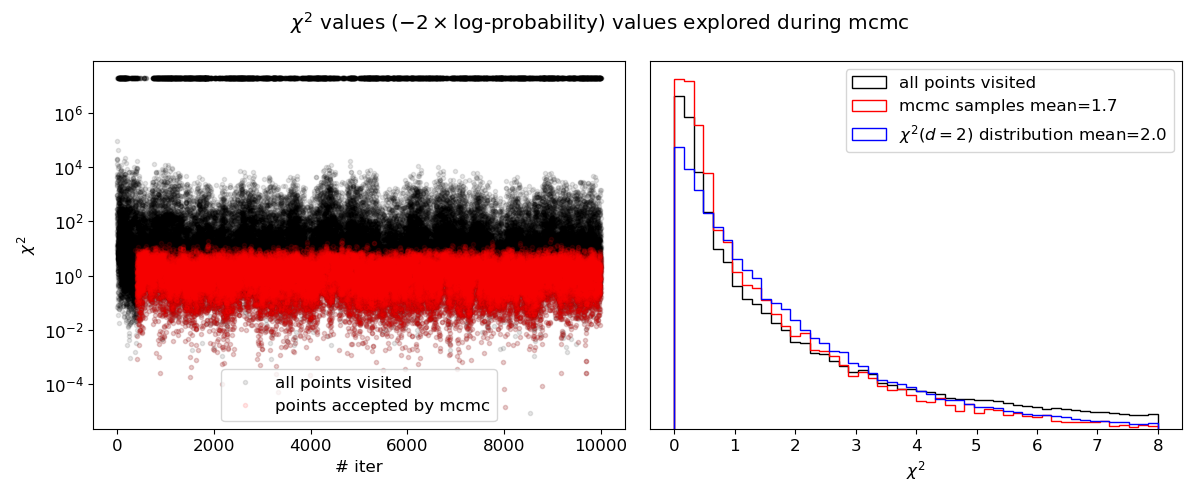
\includegraphics[width=\linewidth]{example_mcmc_log_probability_values_explore.png}
  \caption{The evolution of $\chi^2 = -2\log p$ during the run, and the histogram of accepted
           values (red) against a $\chi^2$ distribution with two degrees of freedom (blue). The
           numerically computed means are given in the legend; the analytic mean of the $\chi^2$
           distribution is the dimension.}
\end{figure}

The final product of the analysis is a \href{https://github.com/dfm/corner.py}{\texttt{corner}}
plot of the posterior, and its stability along the chain:

\begin{figure}[H]
  \centering
  \includegraphics[width=0.62\linewidth]{example_mcmc_parameters_distribution.png}
  \caption{The posterior: one- and two-dimensional marginals.}
\end{figure}

\begin{figure}[H]
  \centering
  \includegraphics[width=0.62\linewidth]{example_mcmc_parameters_distribution_convergence.png}
  \caption{The posterior as it would have been had the chains been stopped at five points along
           the run, from purple (earliest) to red (the full chain).}
\end{figure}

\section{MCMC against grid Monte Carlo}
\label{sec:mcmc-vs-mc}

How much does MCMC actually save? The target is minus the five-dimensional Rosenbrock function of
\cref{eq:rosenbrock}, sampled with $\Nc = 50$ walkers for $\Lc = 5\cdot 10^4$ iterations, starting
close to the known minimum.

\begin{figure}[H]
  \centering
  \includegraphics[width=0.68\linewidth]{example_mcmc_5d_parameters_distribution_convergence.png}
  \caption{The 5D posterior at five stopping points along the chains, without burn-in.}
\end{figure}

\begin{figure}[H]
  \centering
  \includegraphics[width=0.62\linewidth]{example_mcmc_5d_convergence_diagnostics.png}
  \caption{Convergence diagnostics of the 5D run, as in \cref{sec:mcmc-convergence}.}
\end{figure}

The same posterior is then computed by brute force, evaluating the density on a regular grid:

\begin{figure}[H]
  \centering
  \includegraphics[width=0.7\linewidth]{example_mcmc_and_mc_5d_parameters_distribution.png}
  \caption{The 5D posterior from MCMC (black) and from grid Monte Carlo (blue), and from a
           coarser grid with about as many samples as the MCMC (red). The legend gives the total
           number of samples and the computation time of each.}
\end{figure}

\begin{keypoint}[What the comparison shows]
The fine grid needs about $40\times$ more evaluations than MCMC for the same distribution, although
its total time was only about $2.5\times$ longer here, because MCMC carries more algorithmic
overhead per sample. Given the \emph{same} number of samples, the coarse grid is far from converged.
The gap widens rapidly with dimension --- and when each evaluation is an expensive simulation, it is
the number of evaluations, not the overhead, that counts.
\end{keypoint}

\chapter{MCMC with a surrogate model}
\label{ch:surrogate}

\section{The idea}

MCMC needs many evaluations --- tens of thousands even in the small examples of \cref{ch:mcmc}.
When each one is an expensive simulation, that can be out of reach even on a cluster. The
alternative is to train a fast \emph{surrogate} (or emulator) of the log-probability on a modest
number of expensive evaluations, and to run the MCMC on the surrogate instead. Once a fast surrogate
exists, the MCMC no longer needs a cluster, or this package: it can be run with any MCMC library,
such as \texttt{emcee} or \texttt{pymc}.

The difficulty is where to put the training data. Sampling the parameter space at random, over a
domain wide enough to be safe, spreads the evaluations thinly. Standard checks of the surrogate,
such as cross-validation on held-out points, then measure its accuracy \emph{on average over that
domain} --- while what matters is its accuracy on the posterior, a region not known in advance and
typically a small fraction of the domain.

This is where a short expensive MCMC is useful even when a full one is unaffordable: its walkers
generate training data exactly where the posterior is. A surrogate-based calibration therefore
proceeds in five steps:

\begin{enumerate}[leftmargin=*, label=\textbf{\arabic*.}]
  \item Start a parallel MCMC with the expensive function.
  \item Run it long enough to generate relevant training data.
  \item Train a fast surrogate on the evaluations, and test its accuracy.
  \item Run the MCMC on the surrogate; no cluster is needed any more.
  \item Validate the resulting posterior against the expensive function, with importance sampling.
\end{enumerate}

\section{Validating with importance weights}
\label{sec:importance}

The surrogate posterior $\psur$ can be checked directly against the expensive one, $\pexp$. Draw
points $\theta_i$ from the surrogate-based MCMC samples, evaluate the expensive function there, and
form the ratios
\begin{equation}
  w_i = \frac{\pexp(\theta_i)}{\psur(\theta_i)} = \exp\!\big(\log\pexp(\theta_i) - \log\psur(\theta_i)\big),
  \label{eq:importance-weights}
\end{equation}
the \textbf{importance weights}. Where the surrogate is exact every ratio is the same constant;
their spread measures the surrogate's error, precisely on the points where the posterior has mass.
The weights also correct the surrogate-based estimate: an expectation under the expensive posterior
is the weighted average over the surrogate samples,
\begin{equation}
  \mathbb{E}_{\pexp}[h(\theta)] \;\approx\; \frac{\sum_i w_i\, h(\theta_i)}{\sum_i w_i},
\end{equation}
self-normalised so that the unknown constants of both densities cancel.

\section{Example: a surrogate for the 2D Rosenbrock}
\label{sec:surrogate-example}

The target is again the constrained 2D Rosenbrock of \cref{sec:mcmc-example}, standing in for an
expensive function. A short expensive MCMC runs with $\Nc = 10$ walkers for $\Lc = 2000$ iterations
--- not converged, which is not the point here. A Gaussian-process surrogate of the log-probability
is then trained on 400 distinct points from that run, plus 200 random points inside the constraint
circle, which regularize the surrogate away from the chains.

\begin{figure}[H]
  \centering
  \includegraphics[width=\linewidth]{example_mcmc_surrogate_2d_visualization.png}
  \caption{The expensive and the surrogate log-probabilities (logarithm of the absolute value),
           with the training points in red. The training data concentrate where they are needed.}
\end{figure}

The MCMC is then rerun, with the same settings, on the surrogate:

\begin{figure}[H]
  \centering
  \includegraphics[width=0.5\linewidth]{example_mcmc_surrogate_parameters_distribution.png}
  \caption{The posterior from the expensive MCMC and from the surrogate-based MCMC, after burn-in.
           They are similar, but not identical.}
\end{figure}

For validation, 1000 points are drawn from the surrogate-based samples and evaluated with the
expensive function:

\begin{figure}[H]
  \centering
  \includegraphics[width=0.42\linewidth]{example_mcmc_surrogate_importance_weights.png}
  \caption{The ratio of expensive to surrogate probabilities, the importance weights of
           \cref{eq:importance-weights}, on 1000 surrogate-posterior points.}
\end{figure}

The ratios are close to 1, to within about 1\%, which validates the surrogate for this problem ---
and the weights could now be used to correct predictions made from the surrogate-based samples.

\begin{keypoint}[From a manual procedure to an automated one]
Every step above required a judgement: how long to run the expensive MCMC, how many regularization
points to add, whether the surrogate is accurate enough, and what to do if it is not. The hybrid
pipeline of \cref{ch:hybrid} iterates the procedure, measures its accuracy on the posterior after
each iteration, recycles the validation evaluations as new training data, and stops when measured
criteria are met.
\end{keypoint}

\chapter{The automated hybrid surrogate-MCMC pipeline}
\label{ch:hybrid}

The procedure of \cref{ch:surrogate} works, but leaves every decision to the user and gives no
guarantee at the end. \code{slurm_mcmc_hybrid} automates it: it iterates fit, sample and validate
until measured criteria say the surrogate posterior can be trusted, recycling every expensive
evaluation it makes along the way.

\section{The loop}
\label{sec:hybrid-loop}

\begin{enumerate}[leftmargin=*, label=\textbf{\arabic*.}]
  \item \textbf{Round 0.} A \emph{short} expensive MCMC, plus optional
        \code{num_regularization_points}, generates the initial training set. Its walkers --- the
        parallel MCMC chains of \cref{ch:mcmc} --- are evaluated in parallel on the cluster, so
        their number is this stage's parallelism. The regularization points are the only
        evaluations in the whole run placed without reference to a posterior, and so the only ones
        that can find mass the surrogate does not already know about.
  \item \textbf{Fit} a fast surrogate: a Gaussian process by default (\cref{sec:hybrid-surrogates}).
  \item \textbf{Sample} the surrogate with a cheap, vectorized MCMC that needs no cluster, confined
        to \code{param_bounds} or, by default, to an envelope grown from the training data
        (\cref{sec:unbounded}). A fresh sampler is built every round, because each round samples a
        different surrogate, with its own deliberately small set of walkers. This chain is kept
        cheap, because its posterior is discarded at the next fit.
  \item \textbf{Validate.} Evaluate the expensive function, in parallel, on
        \code{num_validation_points} drawn from the surrogate posterior, and score the criteria of
        \cref{sec:hybrid-measured}.
  \item \textbf{Refine.} If the criteria are not met, the validation evaluations --- which sit
        exactly where the surrogate needs improving, and are already paid for --- join the training
        set, and the loop returns to step 2. Optionally, each round also runs a few expensive MCMC
        steps started from the current surrogate posterior (\code{num_expensive_iters_per_round}).
  \item \textbf{Verify.} A pass reached on a cheap chain is only provisional. The same surrogate is
        re-sampled to reporting depth (\cref{sec:two-depths}) and one more validation batch is
        spent on \emph{that} posterior. If it still passes, it is the posterior returned; if not,
        refinement resumes. No evaluation is wasted either way: the refinement batch joins the
        training set as soon as verification starts, and a rejected verification's batch joins it
        too.
\end{enumerate}

Verification buys two things. The returned posterior is sampled properly, rather than being
whatever a deliberately cheap chain happened to produce. And the decision to stop rests on two
independent measurements rather than one --- which matters, because a single measurement from 100
validation batch is noisy: two batches scored against the \emph{same} surrogate can land on opposite
sides of the threshold.

\begin{keypoint}[Starting from existing evaluations]
If expensive evaluations already exist --- from an ordinary \code{slurm_mcmc} run, a parameter scan,
an earlier study --- pass them as \code{initial_train_points} and \code{initial_train_values}. Round 0
is skipped and the first surrogate is fitted on them directly; \code{init_points} is then not needed,
and the evaluations do not count towards \code{num_expensive_evals}, which records only what the run
itself spent. The regularization points are part of round 0, so they are skipped too, with a warning.
\begin{lstlisting}
pool = status['slurm_pool']                 # from a previous slurm_mcmc
result = slurm_mcmc_hybrid(..., initial_train_points=pool.points_history,
                           initial_train_values=pool.values_history[:, 0])
\end{lstlisting}
\end{keypoint}

\section{What is measured}
\label{sec:hybrid-measured}

On the validation points $\theta_i$, write the log-ratio of the expensive to the surrogate
log-probability, and the self-normalised importance weights of \cref{sec:importance}:
\begin{equation}
  d_i = \log\pexp(\theta_i) - \log\psur(\theta_i),
  \qquad w_i = e^{d_i},
  \qquad \tilde w_i = \frac{w_i}{\sum_j w_j}.
\end{equation}
The weights are the \emph{ratio}, not the expensive density, because the points were drawn from the
surrogate posterior and so already arrive with density $\propto \psur$: the sampling density has to
be divided out before the target density is multiplied in.

\begin{keypoint}[Nats]
Every logarithm here is natural, and the unit of a log-probability is the \emph{nat} --- which is
what ``[nats]'' means on the figures below. A difference of $\Delta$ nats in log-probability is a
factor $e^{\Delta}$ in probability: 1~nat is a factor of 2.7, 0.1~nats about 10\%, and 0.01~nats
about 1\%.
\end{keypoint}

\subsection{Surrogate accuracy}

\begin{equation}
  \bar d = \sum_i \tilde w_i\, d_i,
  \qquad
  \varepsilon = \sqrt{\sum_i \tilde w_i\, (d_i - \bar d)^2}\quad[\text{nats}].
  \label{eq:epsilon}
\end{equation}
$\varepsilon = 0.05$ means probability ratios are accurate to about 5\%. The mean $\bar d$ is
subtracted because a log-probability is only defined up to a constant, so only the \emph{spread} of
$d$ is a real error. The weighting makes $\varepsilon$ an average under the \emph{expensive}
posterior: an error where the true probability is high counts far more than the same error in the
tails.

\subsection{Degeneracy guard}

$\varepsilon$ alone is not safe. If the weights collapse onto a few points, it is computed from
those points alone and can be arbitrarily small --- exactly zero for a single dominating point ---
while the surrogate is in fact terrible. The number of validation points that effectively carry the
weight is
\begin{equation}
  \ESSw = \frac{\left(\sum_i w_i\right)^2}{\sum_i w_i^2} \in [1, N],
\end{equation}
and a run is never declared converged while $\ESSw <$ \code{min_ess_weights}. $\ESSw$ counts
validation points and is unrelated to the ESS of a chain, $N/\tau$, of \cref{eq:ess}.

\subsection{Posterior stability}

Surrogate accuracy and posterior convergence are different questions: a perfect surrogate still
leaves a drifting posterior if its chain is too short. Between rounds, the change in each
parameter's posterior mean $m_j$ and standard deviation $s_j$ is measured in units of that
parameter's posterior width, and the largest is kept:
\begin{equation}
  \delta = \max_j
  \frac{\max\!\left(\,\big|m_j^{\mathrm{new}} - m_j^{\mathrm{old}}\big|,\ \big|s_j^{\mathrm{new}} - s_j^{\mathrm{old}}\big|\,\right)}
       {\tfrac12\left(s_j^{\mathrm{new}} + s_j^{\mathrm{old}}\right)} .
  \label{eq:delta}
\end{equation}
$\delta = 0.1$ means nothing moved by more than a tenth of a posterior width --- a statement about
the answer rather than about the chain. Two estimates of the \emph{same} posterior still differ by
chance, by roughly $\sqrt{1/\ESS_{\mathrm{new}} + 1/\ESS_{\mathrm{old}}}$ widths, where ESS is the
chain's and ``old'' is the previous round's reported posterior. The tolerance actually applied
therefore never drops below three times that noise floor:
\begin{equation}
  \delta \;\le\; \max\!\left(\texttt{posterior\_shift\_tolerance},\;
  3\sqrt{\frac{1}{\ESS_{\mathrm{new}}} + \frac{1}{\ESS_{\mathrm{old}}}}\right).
  \label{eq:stability}
\end{equation}
Without the floor a tolerance of 0.1 would be unreachable at realistic chain depths: at the ESS of
95--380 in the worked example, the floor alone is 0.23--0.42. The test needs two rounds, so a run
cannot converge in round 1 while it is enabled; \code{posterior_shift_tolerance=None} switches it
off.

\subsection{The convergence test}

All three conditions must hold simultaneously:
\begin{gather}
  \varepsilon \le \texttt{log\_error\_threshold},
  \qquad
  \ESSw \ge \texttt{min\_ess\_weights},
  \notag\\
  \delta \le \max\!\left(\texttt{posterior\_shift\_tolerance},\ \text{noise floor}\right).
\end{gather}

\begin{cautionbox}[What the test cannot see]
Every statistic is evaluated on points drawn from the \emph{surrogate} posterior. The test therefore
detects a surrogate posterior that is too \textbf{broad}, and cannot detect one that is too
\textbf{narrow}: mass the surrogate never finds is never sampled, never scored, and never enters any
statistic. The worked example below misses a tail in exactly this way. If the target may be
hierarchical or multimodal, spend some budget on \code{num_regularization_points}, disperse
\code{init_points}, and consider an independent short expensive chain as a check.
\end{cautionbox}

\section{Two sampling depths}
\label{sec:two-depths}

The two chain criteria of \cref{sec:mcmc-convergence} are applied at two depths. The surrogate
chain runs \code{num_surrogate_iters} iterations, and is extended in blocks of that size, on the same
sampler, until the criteria of its tier hold --- or \code{max_surrogate_iters_multiplier} blocks
have been spent, which is logged as a warning.

\begin{center}
\small
\begin{tabularx}{\linewidth}{@{}l L L@{}}
  \toprule
  & \textbf{refining} --- posterior discarded at the next fit & \textbf{verifying} --- posterior reported \\
  \midrule
  effective samples, $N/\tau$ & \code{refine_surrogate_ess}: \code{None} $\to 10\,d$ & \code{final_surrogate_ess}: \code{None} $\to 100\,d$ \\
  chain length, $\Lc/\tau$    & \code{refine_iters_per_tau}: \code{None} $\to$ not demanded & \code{final_iters_per_tau}: $50$ \\
  \bottomrule
\end{tabularx}
\end{center}

The defaults are the two ends of the advised band of $10$--$100\times d$. The length criterion is not
demanded while refining, for two reasons: that posterior is discarded, and $\tau$ cannot be measured
reliably on a short chain anyway --- that is what $\Lc \ge 50\tau$ \emph{means} --- so a floor on it
would be enforced against a number that is itself unreliable. Samples and $\tau$ are always taken
after discarding \code{surrogate_burnin_fraction} of the chain.

\code{max_verification_attempts}, by default \code{None}, lets a failed verification send the run
back to refining as often as the target needs, since \code{num_rounds_max} bounds it anyway. A finite
cap means \emph{give up after this many rejections} and ends the run: a run that can no longer
verify can never converge. \code{0} switches verification off.

\section{Surrogate models}
\label{sec:hybrid-surrogates}

\code{surrogate} accepts one of the following, or any object with \code{fit(X, y)} and
\code{predict(X)} --- and \code{predict_std(X)} too, if the uncertainty penalty should be active:

\begin{itemize}
  \item \textbf{\code{'gp'}} (default), a \code{GaussianProcessSurrogate} --- the recommended choice:
        accurate, smooth, and it reports its own uncertainty.
  \item \textbf{\code{'polynomial'}}, a \code{PolynomialSurrogate} --- a cheap fallback for
        posteriors that really are low-order. It extrapolates badly otherwise, and has no
        uncertainty, so the uncertainty penalty is inactive with it.
  \item \textbf{\code{DistributedGPSurrogate(...)}} --- an ensemble of Gaussian processes, for when
        the training set has grown too large for a single one to be refitted every round.
\end{itemize}

The first two wrap standard scikit-learn models:
\code{GaussianProcessRegressor} for the Gaussian process, and a ridge regression on polynomial
features for the polynomial. The Gaussian process first fits a polynomial mean function, so that the
process only has to model what the polynomial misses. The third,
\code{DistributedGPSurrogate}, is not a standard model, and is described in \cref{sec:rbcm}.

\subsection{The uncertainty penalty}

During the surrogate MCMC the surrogate is evaluated pessimistically, as
\begin{equation}
  \log\psur(\theta) = \mu(\theta) - \kappa\, \sigma(\theta),
\end{equation}
where $\mu$ and $\sigma$ are its prediction and uncertainty and $\kappa$ is
\code{surrogate_uncertainty_penalty}. A Gaussian process's uncertainty grows away from its training
data, so walkers are turned back from regions where the surrogate would be extrapolating.

\subsection{DistributedGPSurrogate}
\label{sec:rbcm}

\textbf{Why it exists.} The surrogate is refitted every round on the whole training set, and the
cost of fitting a Gaussian process grows steeply --- roughly with the cube of the number of points.
Early in a run that is negligible, but every round adds evaluations, so on a long run the fit comes
to dominate and eventually stops being affordable at all. \code{DistributedGPSurrogate} is the way
past that point.

\textbf{What it does.} It is a robust Bayesian Committee Machine (Deisenroth \& Ng 2015, with Cao \&
Fleet's 2014 weights). It splits the training set among independent Gaussian-process
\emph{experts} and recombines their predictions in closed form. It attacks cost by parallelism
rather than approximation: the expert fits are independent, so on a cluster the wall clock is that of
a single expert.

At any point, every expert predicts a value and an uncertainty, and the ensemble takes a weighted
average of the values. An expert's weight is how much it has learned at that point: how far its
uncertainty there has fallen below the uncertainty it had before seeing any data. An expert sitting
on its own training points is confident and dominates; an expert far from them is back where it
started and gets no weight at all. The weights add up to one, so a single expert reproduces itself
exactly --- a one-expert ensemble \emph{is} the dense Gaussian process --- and where no expert has
learned anything, the ensemble falls back to the experts' starting uncertainty, which is large. That
large uncertainty is what keeps the uncertainty penalty working away from the data. Each expert is
judged against the uncertainty \emph{it} started with: experts routinely settle on scales far from
the nominal one, and judging them against it would make every expert look uninformed away from its
data.

\begin{argtable}
  \code{max_points_per_expert} & \code{None} & set this for large training sets: it grows the \emph{number} of experts with the data instead of the size of each, which keeps fitting affordable \\
  \code{num_experts} & \code{8} & the number of experts, when \code{max_points_per_expert} is not set \\
  \code{min_points_per_expert} & \code{200} & below this many points per expert, fewer experts are used, down to one; an expert fitted on a few dozen points cannot identify its own kernel \\
  \code{partition} & \code{'kmeans'} & how points are split: \code{'kmeans'} (spatial clusters) or \code{'random'} \\
  \code{n_restarts_optimizer} & \code{2} & restarts of each expert's hyperparameter fit; more give better fits for little cost \\
  \code{parallel} & \code{'none'} & \code{'joblib'}: one process per core; \code{'slurm'}: one job array across nodes, worth it only when a single expert fit is long compared with the queue wait \\
  \code{n_jobs}, \code{cluster}, \code{submitit_kwargs} & \code{-1}, \code{'slurm'}, \code{None} & settings of the \code{'joblib'} and \code{'slurm'} modes \\
  \code{work_dir} & \code{None} & scratch location for \code{'slurm'}, \code{work_dir/surrogates/dgp_experts}, removed once the experts are back; inherited from the pipeline's, and must be on a shared filesystem \\
  \code{job_name} & \code{None} & for \code{'slurm'}, the expert job arrays are named \code{job_name_dgp_fit<n>}; inherited from the pipeline's \\
  \code{max_fit_retries} & \code{2} & failed expert jobs are retried individually, then fitted locally \\
  \code{trend_degree} & \code{2} & the polynomial mean function, as for the dense Gaussian process \\
\end{argtable}

Two behaviours are worth knowing. The prediction cannot be computed without the uncertainties,
because the weights come from them, so turning the uncertainty penalty off saves the ensemble
nothing. And cost moves rather than disappears: every MCMC step queries all the experts, so fitting
becomes nearly free while sampling becomes the dominant cost, and end to end the ensemble can be
slower than the dense Gaussian process even though it fits far faster. It pays once the dense fit
itself is the bottleneck.

\section{Training data}

The training set only grows: every expensive evaluation is kept. What enters each fit can be
limited. \code{train_log_prob_trim_range} drops points more than that many nats below the best
one --- their probability is $e^{-100}$ at the default, so no MCMC will ever visit them, and they only
make the fit more expensive --- as long as at least \code{min_train_points_after_trim} points remain.
Below about 20 nats accuracy collapses, because the surrogate then has no evidence that the
probability is low away from the peak. \code{max_train_points} caps the fit with a uniform random
subsample, which preserves spatial coverage; keeping the highest-probability points instead would
discard exactly the far-field points that stop the surrogate extrapolating. \code{train_log_prob_floor}
drops points below an absolute value, such as penalty or failure values.

\section{Running without bounds}
\label{sec:unbounded}

\code{param_bounds} defaults to \code{None}, and then no box is imposed. A box cannot simply be
dropped, though, because a surrogate says nothing reliable away from its training data, and both ways
it can be wrong there are fatal to an MCMC: with a fitted quadratic trend the surrogate tends to that
quadratic, which runs off to $+\infty$ along any direction of positive curvature; without a trend it
tends to a constant, which is improper over infinite volume. Either way the chain walks away and
never returns.

So the training set's own geometry decides where the surrogate may be believed. Let $r(\theta)$ be
the Mahalanobis radius of $\theta$ under the training points' mean and covariance, and $R$ the largest
such radius among them. A quartic penalty switches on beyond $2R$, and the log-probability is
$-\infty$ beyond $10R$, which makes the posterior proper outright. Nothing acts inside $2R$, so the
posterior over the data is untouched; and because both radii are multiples of $R$, they grow as
evaluations accumulate outwards, so a genuinely long tail is followed round after round.

With the default Gaussian process the envelope never actually fires: its uncertainty grows away from
the data, so the uncertainty penalty turns the walkers back long before the envelope --- on the
worked example, the largest radius the walkers reached was 3.51 with the envelope switched on and off
alike. It is load-bearing only for surrogates without an uncertainty, such as the polynomial.

\needspace{22\baselineskip}
\section{Usage}
\label{sec:hybrid-usage}

\begin{lstlisting}
import numpy as np
from slurmcmc.hybrid import slurm_mcmc_hybrid

def log_prob(theta):                            # the expensive log-probability
    ...

num_params = 3
init_points = np.random.uniform(-2, 2, (10 * num_params, num_params))   # round-0 walkers

result = slurm_mcmc_hybrid(log_prob_fun=log_prob, init_points=init_points,
                           num_expensive_iters=10, num_regularization_points=50,
                           log_error_threshold=0.01, num_rounds_max=30,
                           cluster='slurm', work_dir='hybrid',
                           save_restart=True, random_seed=0)

print(result['converged'], result['num_rounds'], result['num_expensive_evals'])
samples = result['samples']                     # the posterior, as flat draws
\end{lstlisting}

Most arguments can stay at their defaults. The ones that decide a run are its round-0 budget ---
the number of walkers in \code{init_points}, \code{num_expensive_iters} and
\code{num_regularization_points} --- the accuracy it must reach, \code{log_error_threshold}, and
how many rounds it may take, \code{num_rounds_max}. To start from evaluations that already exist,
pass \code{initial_train_points} and \code{initial_train_values} instead of \code{init_points}
(\cref{sec:hybrid-loop}); to use another surrogate, pass \code{surrogate}
(\cref{sec:hybrid-surrogates}). With \code{remote=True} the call returns a submitit job, and
\code{result = job.result()} gives the same dictionary (\cref{sec:remote}).

\code{example_mcmc_hybrid.py} spells out every argument on its own line and is the best starting
point for a real problem; \cref{sec:hybrid-args} describes them all, and the returned dictionary is
described at the end of this chapter.

\section{Worked example: a 3D Rosenbrock}
\label{sec:hybrid-example}

This is exactly what \code{example_mcmc_hybrid.py} does, so every number below is reproducible by
running it. The target is minus the 3D Rosenbrock function of \cref{eq:rosenbrock}: a narrow,
curved, banana-shaped posterior. Because it is analytic, a plain expensive MCMC on it is affordable,
and that gives a reference to judge the hybrid run against --- so the reference comes first.

\subsection{The expensive reference}

The reference is a plain \code{slurm_mcmc} on the same target, with no surrogate anywhere: 100\,000
iterations with 30 walkers, \textbf{3\,000\,000 evaluations}. It is cached separately from the
pipeline's results, so changing a hybrid setting does not pay for it again. A reference is only a
yardstick once it has converged itself, so the example draws its posterior at five points along the
chain, after discarding the first 20\% as burn-in.

\begin{figure}[H]
  \centering
  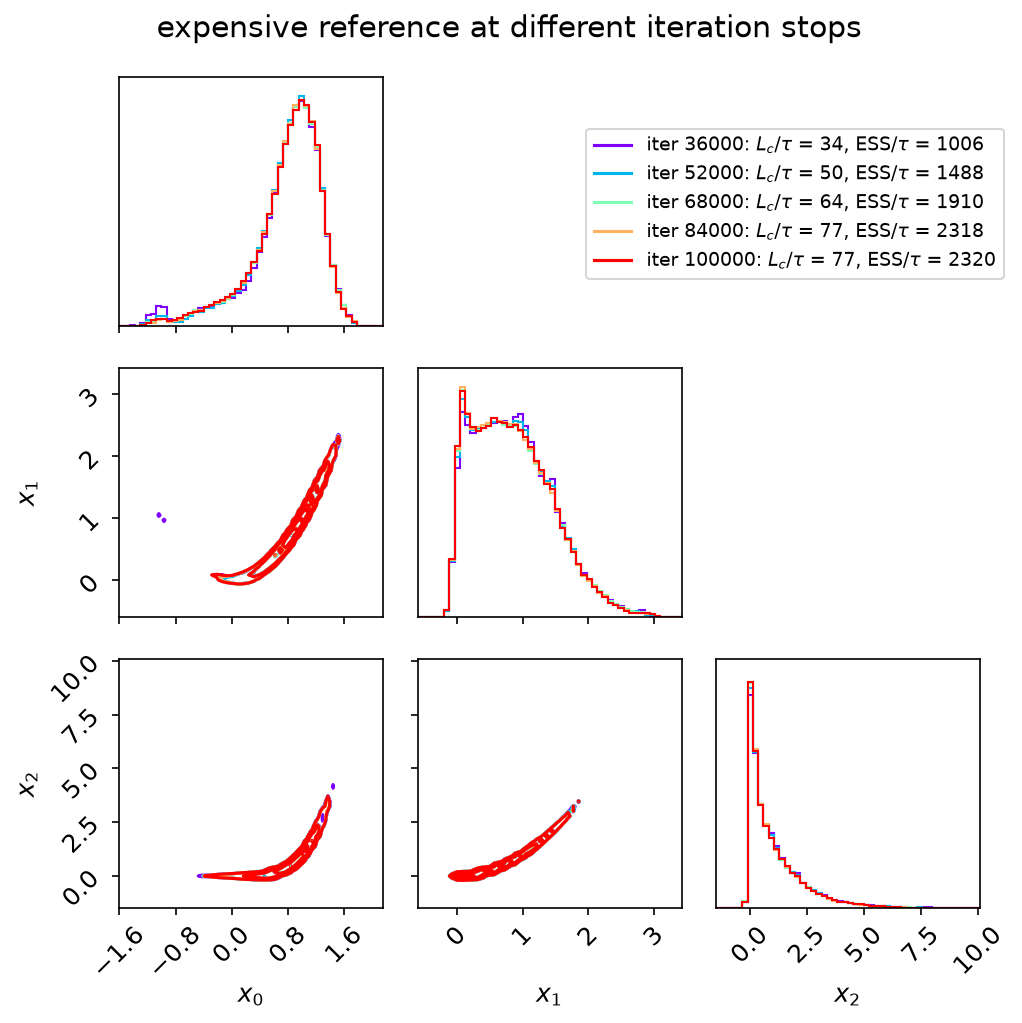
\includegraphics[width=0.5\linewidth]{example_mcmc_hybrid_reference_convergence.png}
  \caption{The reference posterior at five stopping points along the chain, with $\Lc/\tau$ and
           the effective sample size for each in the legend. The figures label the effective sample
           size ESS/$\tau$, for the number of samples divided by $\tau$; $\tau$ is the largest over
           the parameters.}
  \label{fig:hybrid-reference}
\end{figure}

\begin{center}
\small
\begin{tabular}{@{}rrlrr@{}}
  \toprule
  \textbf{stop (iteration)} & $\Lc$ & $\tau$ \textbf{per parameter} & $\Lc/\tau$ & \textbf{ESS} \\
  \midrule
  36\,000  & 16\,000 & 477, 441, 473    & 34 & 1\,006 \\
  52\,000  & 32\,000 & 645, 481, 529    & 50 & 1\,488 \\
  68\,000  & 48\,000 & 754, 533, 617    & 64 & 1\,910 \\
  84\,000  & 64\,000 & 828, 560, 649    & 77 & 2\,318 \\
  100\,000 & 80\,000 & 1\,035, 589, 685 & 77 & 2\,320 \\
  \bottomrule
\end{tabular}
\end{center}

The distributions agree from the third stop on, and $\Lc/\tau$ clears 50. But the caveat of
\cref{sec:mcmc-convergence} applies: $\Lc/\tau$ only means something once $\tau$ has stopped
growing, and $\tau(x_0)$ has not --- its last step is the largest. The cause is a long arm of the
posterior at negative $x_0$: walkers enter it rarely (about 8\% of the mass lies at $x_0 < 0$), and a
single visit can last over 13\,000 iterations, so the longer the chain, the longer the excursions it
has seen. The moments are stable within their error bars, so the comparison below stands, but the
reference's own uncertainty on the width in $x_0$ may be understated.

\subsection{The hybrid run}

A Gaussian-process surrogate with the default quadratic mean function. The settings that differ from
the library defaults:

\begin{center}
\small
\begin{tabularx}{\linewidth}{@{}>{\raggedright\arraybackslash}p{0.40\linewidth}>{\raggedright\arraybackslash}p{0.12\linewidth}L@{}}
  \toprule
  \textbf{setting} & \textbf{value} & \textbf{why} \\
  \midrule
  expensive walkers, \code{len(init_points)} & $10\,d = 30$ & the cluster parallelism of the expensive stage \\
  \code{num_expensive_iters}, \code{num_regularization_points} & 10, 50 & a deliberately small round-0 budget, so refinement has work to do \\
  \code{num_surrogate_iters}, \code{max_surrogate_iters_multiplier} & 5\,000, 30 & room for the verification chain to reach reporting depth \\
  \code{log_error_threshold} & 0.01 & demanding, so the loop refines for several rounds \\
  \code{posterior_shift_tolerance} & \code{None} & stability not tested: the run stops on accuracy alone \\
  \code{num_rounds_max} & 30 & this target needs more than a handful \\
  \code{save_posterior_samples} & 2\,000 & keeps each round's posterior \\
  \bottomrule
\end{tabularx}
\end{center}

\begin{keypoint}[Result]
Converged in \textbf{7 rounds on 1\,380 expensive evaluations}, about 16 minutes --- 0.05\% of the
reference's evaluations. Three verification pushes were spent; two were rejected.
\end{keypoint}

\subsection{Convergence, round by round}

The posterior shift is in units of \textbf{posterior standard deviations} --- the ``[sd]'' on its
axis and in the table below. It is $\delta$ of \cref{eq:delta}: a shift of 0.1 means that, since the
previous round, no parameter's posterior mean or standard deviation moved by more than a tenth of that
parameter's posterior standard deviation.

A verified round has \textbf{two rows}: $n$ for the refinement chain, whose metrics passed and so
triggered the verification, and $n$v for the verification chain that then judged it. $n_{\mathrm{exp}}$
counts the expensive evaluations accumulated before the round, and $n_{\mathrm{train}}$ those that
entered the fit; the two rows share one fit, so both are given on the first row only.

\begin{figure}[H]
  \centering
  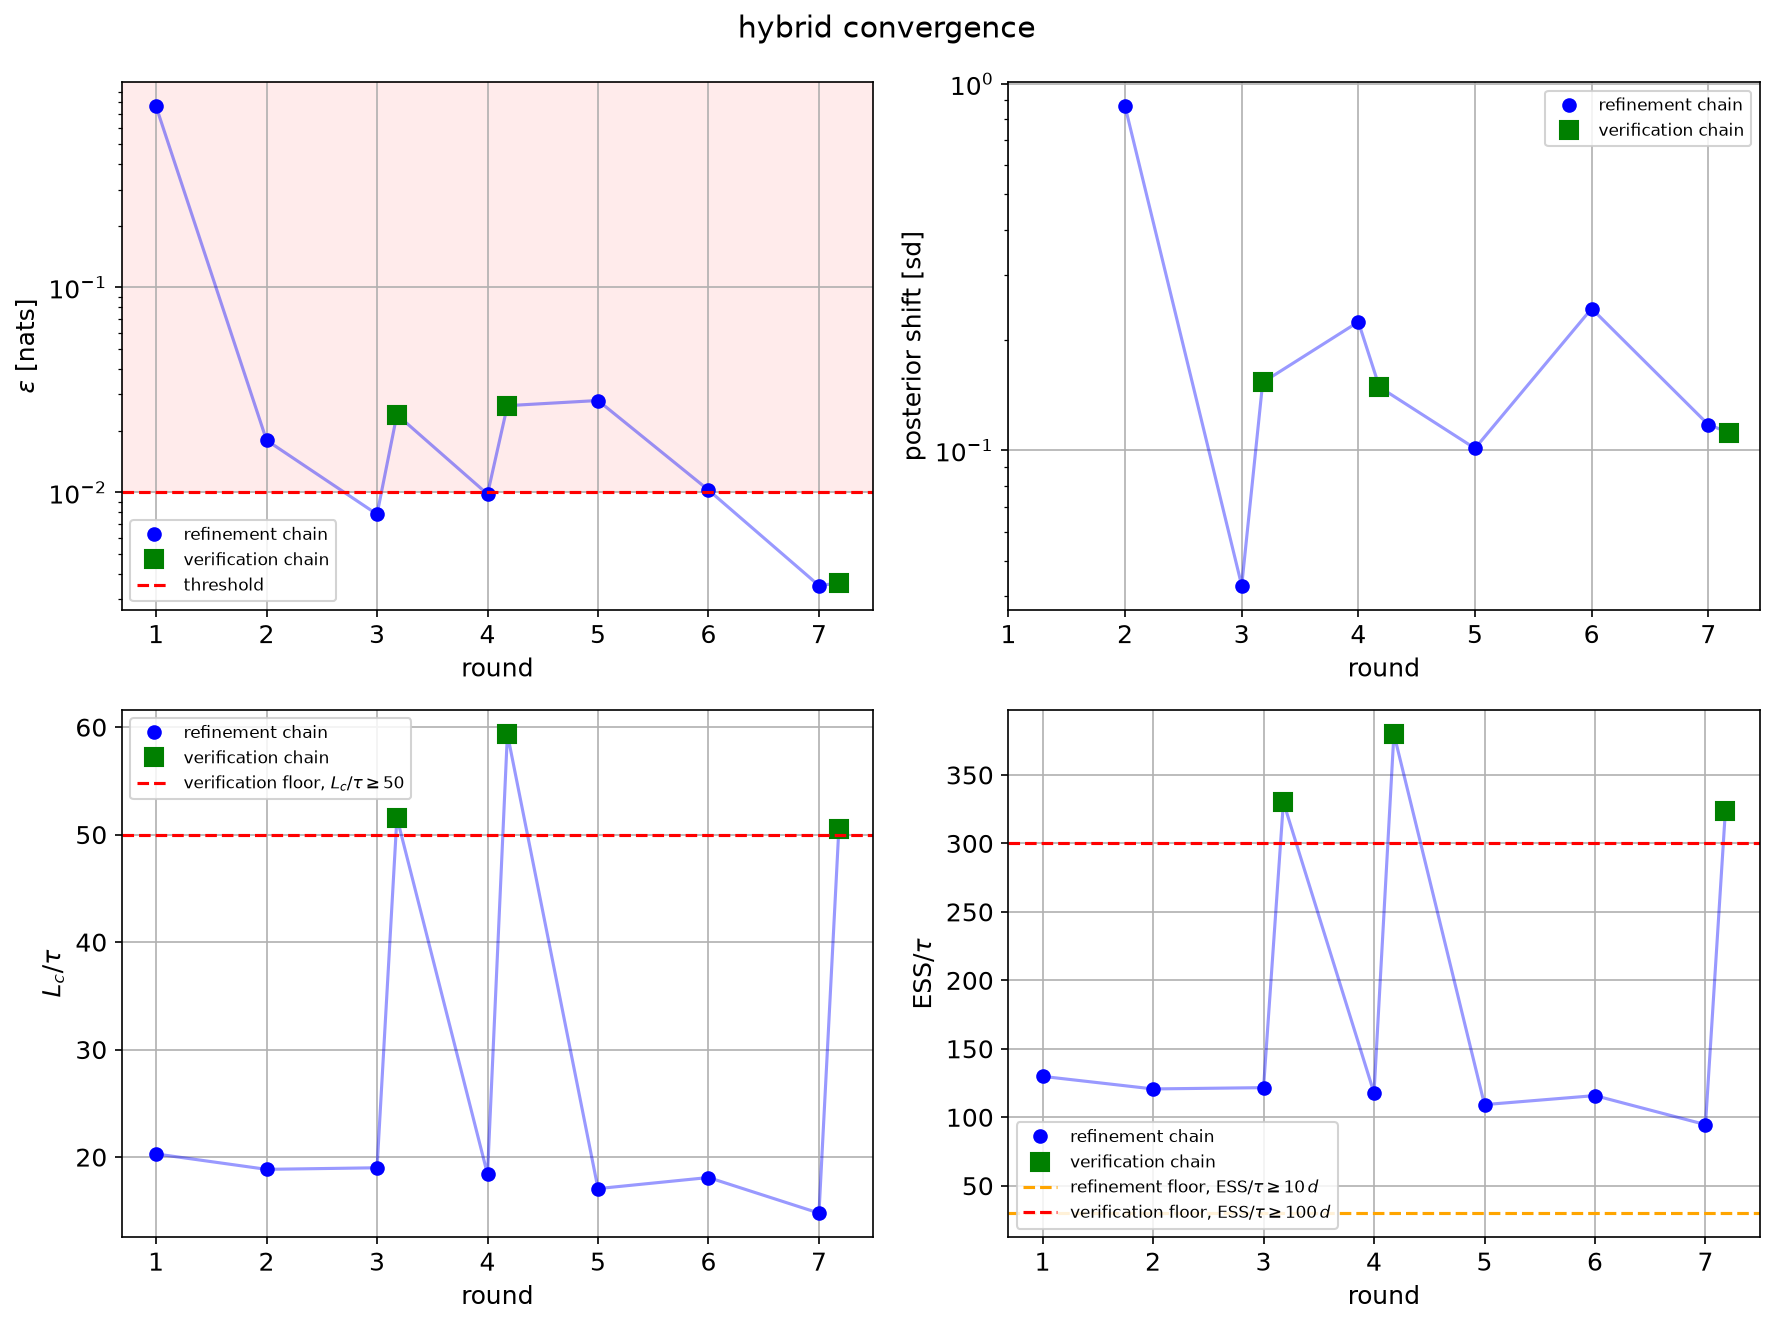
\includegraphics[width=\linewidth]{example_mcmc_hybrid_convergence.png}
  \caption{Top: the criteria, surrogate accuracy $\varepsilon$ and posterior shift $\delta$, with
           the region a converged run must stay out of shaded. Bottom: how deeply the surrogate
           chain was sampled, $\Lc/\tau$ and ESS against their floors. Green squares are
           verification chains, blue circles refinement chains.}
  \label{fig:hybrid-convergence}
\end{figure}

\begin{center}
\small
\begin{tabular}{@{}lrrrrrrr@{}}
  \toprule
  \textbf{round} & $n_{\mathrm{exp}}$ & $n_{\mathrm{train}}$ & $\varepsilon$ [nats] & $\delta$ [sd] & $\Lc$ & $\Lc/\tau$ & ESS \\
  \midrule
  1  & 380    & 123 & 0.7636 & ---   & 5\,000  & 20.3 & 130 \\
  2  & 480    & 223 & 0.0179 & 0.867 & 5\,000  & 18.9 & 121 \\
  3  & 580    & 323 & 0.0078 & 0.043 & 5\,000  & 19.0 & 122 \\
  3v &        &     & 0.0239 & 0.153 & 20\,000 & 51.6 & 330 \\
  4  & 780    & 523 & 0.0098 & 0.224 & 5\,000  & 18.4 & 118 \\
  4v &        &     & 0.0264 & 0.149 & 40\,000 & 59.4 & 380 \\
  5  & 980    & 723 & 0.0280 & 0.101 & 5\,000  & 17.1 & 109 \\
  6  & 1\,080 & 823 & 0.0102 & 0.243 & 5\,000  & 18.1 & 116 \\
  7  & 1\,180 & 923 & 0.0035 & 0.117 & 5\,000  & 14.8 & 95 \\
  7v &        &     & 0.0036 & 0.112 & 30\,000 & 50.6 & 324 \\
  \bottomrule
\end{tabular}
\end{center}

\begin{itemize}
  \item \textbf{Verification did the deciding work.} Rounds 3 and 4 passed on their refinement
        chains, at $\varepsilon = 0.0078$ and $0.0098$; the \emph{same surrogates}, re-sampled
        properly and scored on fresh batches, gave $0.0239$ and $0.0264$ and were rejected. Round 7
        passed both, and rounds 5 and 6 missed the threshold on their refinement chains. That the
        fresh estimate came out higher each time is expected: a round is only verified when its
        refinement $\varepsilon$ happened to land below the threshold, and a single 100-point
        estimate scatters. A stop decided on one batch is partly luck.
  \item \textbf{The two sampling depths are explicit in the bottom row.} Refinement chains ran the
        minimum 5\,000 iterations at $\Lc/\tau \approx 15$--20, deliberately short of 50, with ESS of
        95--130 against their floor of $10\,d = 30$. The three verification chains were extended to
        20\,000--40\,000 iterations, until both $\Lc/\tau \ge 50$ and ESS $\ge 100\,d = 300$ held.
  \item \textbf{Stability was not tested, so the shift column is for information.} From round 3 on,
        every shift is 0.04--0.24 posterior widths, against a noise floor of 0.23--0.42. Every one
        sits below its floor, so had the default tolerance of 0.1 been on, the run would have taken
        exactly the same path.
  \item \textbf{$n_{\mathrm{exp}}$ against $n_{\mathrm{train}}$ is the trim at work.} The yield
        $n_{\mathrm{train}}/n_{\mathrm{exp}}$ climbs from 32\% in round 1 to 78\% by round 7. Every
        trimmed point comes from round 0: at the last fit, 207 of the 330 points of the short initial
        chain, which set out from dispersed walkers, and all 50 regularization points. Not one
        of the 800 points added after round 0 was trimmed, because they were drawn from the posterior
        itself.
  \item \textbf{A verified round costs 200 evaluations, not 100}, because both the refinement batch
        and the verification batch are recycled into the training set.
\end{itemize}

\subsection{The posterior, round by round}

\begin{figure}[H]
  \centering
  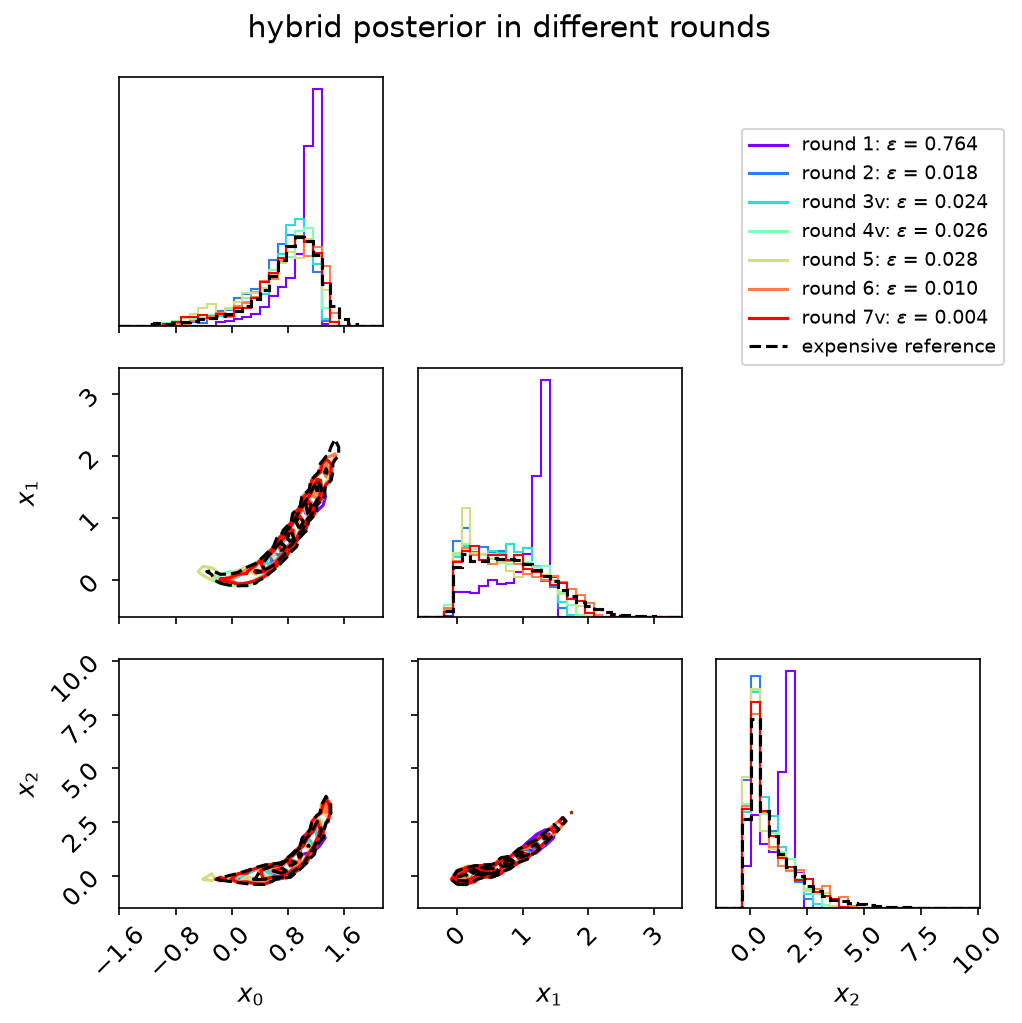
\includegraphics[width=0.82\linewidth]{example_mcmc_hybrid_hybrid_posterior_per_round.png}
  \caption{Each round's posterior as the pipeline left it --- for a verified round, the verification
           chain's --- one colour per round, with the expensive reference dashed in black.}
  \label{fig:hybrid-rounds}
\end{figure}

Round 1 ($\varepsilon = 0.76$) is visibly wrong: a single narrow peak, too high in all three
parameters. From round 2 on the rounds follow the reference's shape, and they reach further into the
long arm at negative $x_0$ as the training data grows: the mass at $x_0 < -0.5$ is 0.6\% in round 2,
1.4\% in round 3, and between 1\% and 4\% after that, against the reference's 2.8\%. What no round
reaches is the other end of the banana, the upper tails of $x_1$ and $x_2$ where the valley climbs
steeply. $\varepsilon$, being measured on points drawn from the surrogate posterior, cannot see a
region the chain never visits. The samples behind the figure are kept in
\code{work_dir/posteriors/round{k}.npy} when \code{save_posterior_samples} is set; nothing else
records them.

\subsection{Where the evaluations went}

\begin{figure}[H]
  \centering
  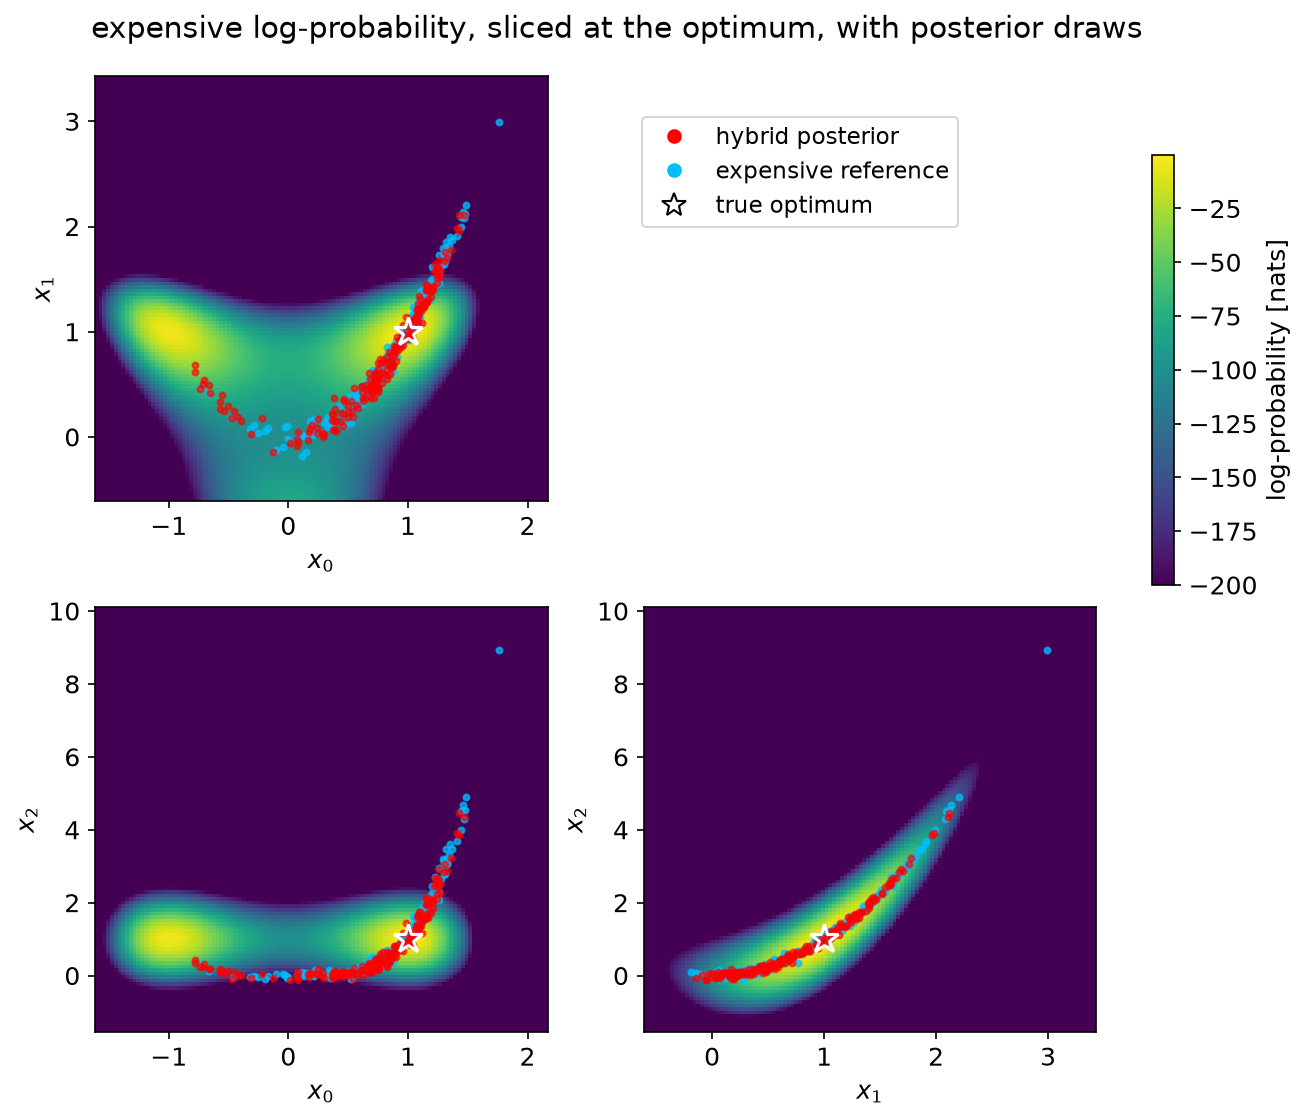
\includegraphics[width=0.96\linewidth]{example_mcmc_hybrid_log_prob_maps.png}
  \caption{The expensive log-probability in each parameter pair, with the remaining parameter held at
           the optimum, and 200 draws each from the hybrid posterior (red) and the reference (light
           blue). The colour scale is in nats, clipped 200 below the peak.}
\end{figure}

The two layers live in different spaces: the background is a \emph{slice} with the remaining
parameter pinned at the optimum, while the dots are a \emph{projection} of the full 3D posterior. A
bright patch with no dots on it, such as the lobe near $x_0 = -1$, is therefore not by itself evidence
of a missed mode. What does matter is visible in the top-left panel: the red draws follow the valley
along the arm at negative $x_0$ down to about $-0.8$, so this run did find it, but at the other end
they stop near $x_1 \approx 2.1$, where the reference continues higher.

\subsection{The posterior against the reference}

\begin{figure}[H]
  \centering
  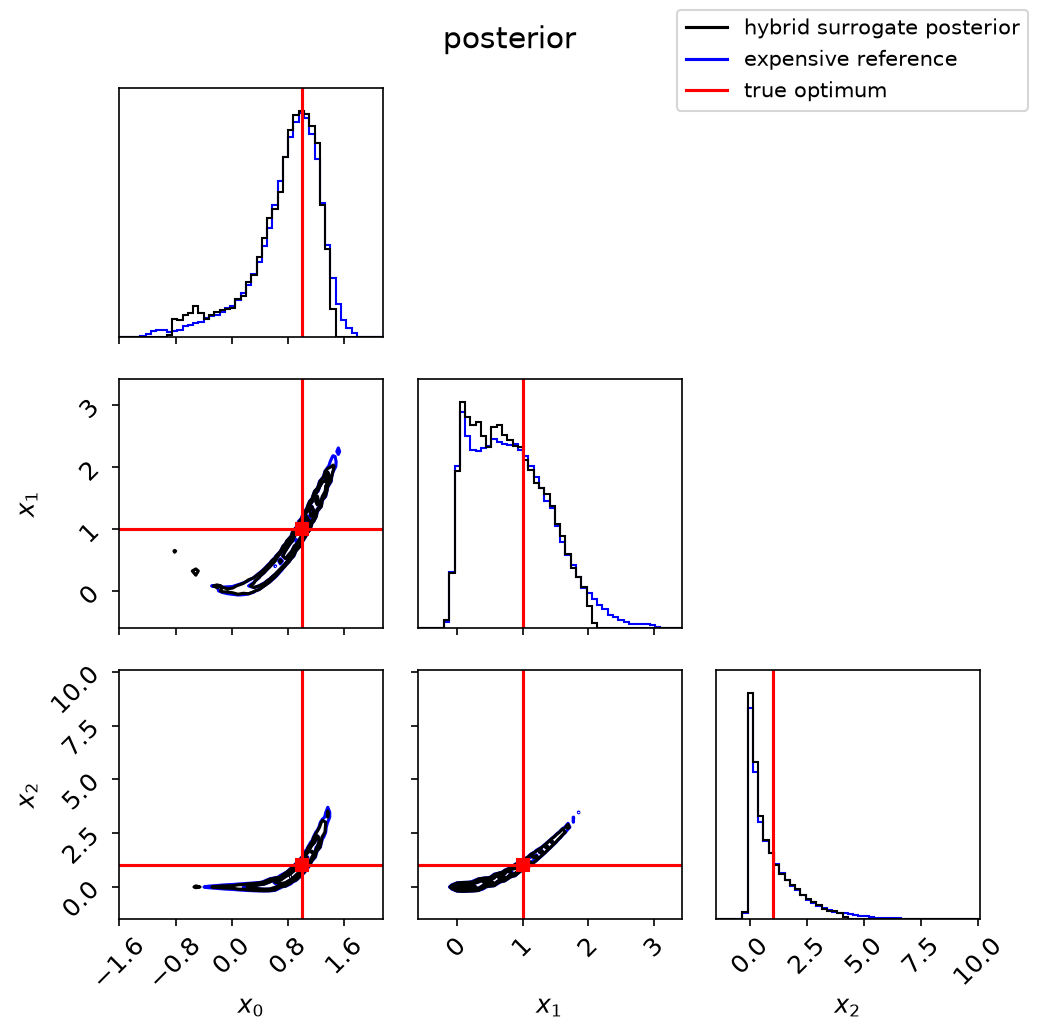
\includegraphics[width=0.82\linewidth]{example_mcmc_hybrid_posterior.png}
  \caption{The hybrid posterior (black) against the expensive reference (blue).}
\end{figure}

\begin{center}
\small
\begin{tabular}{@{}lccc@{}}
  \toprule
  & $x_0$ & $x_1$ & $x_2$ \\
  \midrule
  hybrid standard deviation    & 0.492 & 0.527 & 0.962 \\
  reference standard deviation & $0.493 \pm 0.016$ & $0.594 \pm 0.006$ & $1.296 \pm 0.030$ \\
  hybrid too narrow by         & 0\% & \textbf{11\%} & \textbf{26\%} \\
  \bottomrule
\end{tabular}
\end{center}

The reference's error bars are batch means over ten blocks of 8\,000 iterations. The centres agree
to within 0.14 posterior widths. The width in $x_0$ agrees too: the arm with $x_0 < -0.5$ holds
3.8\% of the hybrid's mass against $2.8\% \pm 0.5\%$ of the reference's. The widths in $x_1$ and
$x_2$ do not, and the upper tails say why: $x_1 > 2$ holds 4.0\% of the reference's mass and 0.4\%
of the hybrid's, and $x_2 > 4$ the same. The run never sampled that end of the banana, so it never
scored it, and every criterion passed regardless. Which tail is cut is partly chance: an earlier run
of this example, on a different random stream, cut the arm at negative $x_0$ as well and came out
31\% too narrow in $x_0$.

\begin{cautionbox}[Reading hybrid widths]
Treat widths and tail quantities from a hybrid run as unconfirmed unless an independent expensive
chain checks them. Means are far more robust than tails.
\end{cautionbox}

\subsection{What the run writes}

For convenience, the run writes \code{work_dir/hybrid_diagnostics.txt} automatically. It is
rewritten in full every round, so a killed run still leaves its complete history and a resumed run
continues the same table. It is reproduced here in part only to explain its content. It opens with
the run's parameters and its evaluation budget:

\begin{lstlisting}[style=plain, basicstyle=\ttfamily\footnotesize]
expensive evaluations
  round 0 MCMC: (num_expensive_iters + 1) * num_walkers = (10 + 1) * 30 = 330
  regularization points: 50
  => raw training points at the first surrogate fit = 330 + 50 = 380
  each refinement round then adds num_validation_points = 100
  (exact unless a proposed point repeats one already evaluated, or an evaluation
   fails, in which case these are upper bounds)
\end{lstlisting}

Each verification spends one more validation batch, which is why this run's total is
$380 + 7 \times 100 + 3 \times 100 = 1\,380$.

A legend describing every column follows, and then the per-round table itself. Here is this run's,
with four columns dropped to fit the page: \code{surrogate}, which names the class fitted that round
and reads \code{GaussianProcess} throughout here, and the timings \code{t_valid_s},
\code{t_refresh_s} and \code{t_round_s} --- the validation batch, the expensive refresh, and the
round total.

\begin{lstlisting}[style=plain, basicstyle=\ttfamily\scriptsize]
round n_expensive n_train w_log_err post_shift surr_iters  Lc/tau  ess/tau  t_fit_s t_mcmc_s
--------------------------------------------------------------------------------------------
    1         380     123    0.7636        inf       5000    20.3      130      2.9     14.3
    2         480     223    0.0179      0.867       5000    18.9      121      2.4     16.4
    3         580     323    0.0078      0.043       5000    19.0      122      7.6     18.5
   3v                        0.0239      0.153      20000    51.6      330              81.0
    4         780     523    0.0098      0.224       5000    18.4      118     20.1     19.4
   4v                        0.0264      0.149      40000    59.4      380             190.6
    5         980     723    0.0280      0.101       5000    17.1      109     42.0     26.1
    6        1080     823    0.0102      0.243       5000    18.1      116     56.9     28.0
    7        1180     923    0.0035      0.117       5000    14.8       95     65.8     30.8
   7v                        0.0036      0.112      30000    50.6      324             226.4
\end{lstlisting}

Reading across a row:

\begin{itemize}
  \item \code{n_expensive} and \code{n_train} are the trim: what has been evaluated, and what
        entered the fit.
  \item \code{w_log_err} and \code{post_shift} are the two criteria, $\varepsilon$ in nats and
        $\delta$ in posterior standard deviations. They are what the run stops on --- here on
        \code{w_log_err} alone, since \code{posterior_shift_tolerance} is \code{None}, but
        \code{post_shift} is computed and printed regardless, so it can be read after the fact.
        The \code{inf} of round 1 marks that there is no previous posterior to compare against yet.
  \item \code{surr_iters}, \code{Lc/tau} and \code{ess/tau} are how deeply the cheap chain was
        sampled: the length actually run, and what it bought in autocorrelation times and effective
        samples. The refinement rows sit at the 5\,000-iteration minimum; the verification rows are
        where \code{surr_iters} jumps to 20\,000--40\,000 until both floors are cleared. A run that
        ends because its chains keep growing without clearing them shows it in these columns.
  \item \code{t_fit_s} against \code{t_mcmc_s} is the pair worth watching. The fit grows with the
        training set, 2.4\,s on 223 points to 65.8\,s on 923, while the cheap MCMC grows with the
        chain length asked of it: the 226.4\,s of round 7's verification is a 30\,000-iteration
        chain on the largest surrogate. On a long run it is the fits, not the sampling, that come to
        dominate --- which is when \code{max_train_points} or a \code{DistributedGPSurrogate}
        becomes worthwhile.
  \item A verified round prints two rows, $n$ and $n$v, and the columns they share ---
        \code{n_expensive}, \code{n_train}, \code{surrogate} and \code{t_fit_s} --- are left empty
        on the second: one fit, one training set, scored twice.
\end{itemize}

\section{Restarting, extending, and changing surrogate}

With \code{save_restart=True}, the restart file is written atomically after round 0 and after every
round, so a crash costs at most the round in progress. It carries the whole training set, which also
makes it the cleanest way to \emph{extend} a finished run: raise \code{num_rounds_max} and resume
with \code{load_restart=True}.

The restart file stores only surrogate-agnostic state --- the training points and their values, the
evaluation count, the per-round diagnostics and the walker positions --- so the surrogate is rebuilt
from whatever is passed on resuming. A run whose fits have become too slow can be stopped and resumed
as an ensemble on the same training data:
\begin{lstlisting}
# start with the dense Gaussian process, for its accuracy
slurm_mcmc_hybrid(..., surrogate='gp', save_restart=True, work_dir='run17')

# fits too slow? stop it, and resume as an ensemble on the same data
from slurmcmc.hybrid import DistributedGPSurrogate
slurm_mcmc_hybrid(..., load_restart=True, save_restart=True, work_dir='run17',
                  num_rounds_max=40,
                  surrogate=DistributedGPSurrogate(max_points_per_expert=500,
                                                   parallel='joblib'))
\end{lstlisting}
Every combination works, in either direction, and the switch is recorded per round. With
\code{save_surrogate}, fitted surrogates are written to \code{work_dir/surrogates/round{k}.pkl}:
\code{'latest'} keeps only the most recent, enough for a resumed round to skip its refit;
\code{'all'} keeps every round, at roughly $8n^2$ bytes each. A saved fit is reused only when the
round, the training-set size and the surrogate class all match.

Either mode also appends one line per fit to \code{work_dir/surrogates/surrogate_log.txt}: the
round, the surrogate class, how many points were accumulated, trimmed, subsampled and fitted, how
long the fit took, and the settings it was built with together with its fitted kernel. Being
appended rather than rewritten, it outlives \code{'latest'} pruning the pickles and continues
across a restart, so it is where a switch of surrogate --- or a fit that is becoming the bottleneck
--- shows up as a sequence.

\section{Results and warnings}

The returned dictionary contains the final posterior \code{samples}; \code{converged},
\code{num_rounds} and \code{num_expensive_evals}; per-round lists of every quantity that decided the
run, including \code{weighted_log_error_per_round}, \code{posterior_displacement_per_round},
\code{surrogate_iters_per_round}, \code{surrogate_tau_per_round}, \code{surrogate_ess_per_round},
\code{verified_per_round} and \code{blocking_criteria_per_round}, which names the criterion that held
each round back; \code{round_records}, one record per measurement including both rows of a verified
round; the fitted \code{surrogate}; the \code{validation_points} and \code{log_importance_weights}
of the final validation; and timings. The emulator's own uncertainty on the validation points,
\code{surrogate_std_per_round}, lets the common assumption that it is negligible be checked rather
than assumed.

Warnings are logged when refinement is not improving fast enough to be worth continuing; when
posterior mass piles up against \code{param_bounds} or the confinement envelope, which can signal a
model error, an unidentifiable parameter or bounds set too tightly; and when a surrogate chain hits its
iteration cap short of its criteria. The stall warning is tuned on \code{HybridMCMCConfig} by
\code{stall_relative_improvement}, \code{stall_window} and \code{stall_significance}.

\section{Argument reference}
\label{sec:hybrid-args}

Arguments shared with the other functions are in \cref{app:common}.

\subsubsection{Starting the run and its expensive budget}
\begin{argtable}
  \code{log_prob_fun} & required & the expensive log-probability; a callable or a deferred-import dictionary \\
  \code{init_points} & \code{None} & starting walkers of the round-0 MCMC, shape $(\Nc, d)$; required unless \code{initial_train_points} is given, and whenever \code{num_expensive_iters_per_round} $> 0$ \\
  \code{param_bounds} & \code{None} & a hard box that constrains the posterior; \code{None} runs unbounded (\cref{sec:unbounded}) \\
  \code{constraint_fun} & \code{None} & feasible when $\le 0$ \\
  \code{num_expensive_iters} & \code{20} & length of the round-0 MCMC; with the walkers, it sets the initial training set, $(\text{iters}+1)\times\Nc$ points \\
  \code{initial_train_points}, \code{initial_train_values} & \code{None} & existing evaluations, shapes $(n, d)$ and $(n)$; round 0 is skipped \\
  \code{num_regularization_points} & \code{0} & points placed without reference to a posterior: uniform in the box, or around the training data when unbounded \\
  \code{num_validation_points} & \code{100} & expensive evaluations per round; sets both the precision of the test and the cost of a round \\
  \code{num_rounds_max} & \code{5} & safety cap on the number of rounds \\
  \code{num_expensive_iters_per_round} & \code{0} & optional expensive MCMC each round, started from the surrogate posterior, costing $(\text{iters}+1)\times\Nc$ evaluations \\
\end{argtable}

\subsubsection{Surrogate and its sampling}
\begin{argtable}
  \code{surrogate} & \code{'gp'} & \code{'gp'}, \code{'polynomial'}, \code{DistributedGPSurrogate(...)}, or any object with \code{fit} and \code{predict} \\
  \code{polynomial_degree} & \code{3} & for \code{surrogate='polynomial'} \\
  \code{surrogate_uncertainty_penalty} & \code{1.0} & $\kappa$ in $\mu - \kappa\sigma$; \code{0} disables \\
  \code{num_surrogate_iters} & \code{2000} & block size of the surrogate chain \\
  \code{max_surrogate_iters_multiplier} & \code{8} & cap on the chain's extension, in blocks \\
  \code{num_surrogate_walkers} & \code{None} & walkers of the surrogate chain; \code{None} is \texttt{emcee}'s minimum, $2d+2$ \\
  \code{surrogate_burnin_fraction} & \code{0.2} & fraction of each chain discarded \\
  \code{refine_surrogate_ess}, \code{final_surrogate_ess} & \code{None}, \code{None} & ESS floors of the two depths; $10\,d$ and $100\,d$ \\
  \code{refine_iters_per_tau}, \code{final_iters_per_tau} & \code{None}, \code{50} & $\Lc/\tau$ floors of the two depths \\
  \code{max_verification_attempts} & \code{None} & rejections allowed before the run gives up \\
\end{argtable}

\subsubsection{Convergence and training data}
\begin{argtable}
  \code{log_error_threshold} & \code{0.1} & $\varepsilon^\ast$ in nats; tighten to 0.01--0.02 for tail quantities \\
  \code{min_ess_weights} & \code{10.0} & the degeneracy guard \\
  \code{posterior_shift_tolerance} & \code{0.1} & $\delta^\ast$ in posterior standard deviations; \code{None} disables \\
  \code{train_log_prob_trim_range} & \code{100.0} & trim points this many nats below the best; \code{None} disables \\
  \code{min_train_points_after_trim} & \code{50} & floor that stops the trim on small training sets \\
  \code{max_train_points} & \code{None} & cap on the fit, by uniform random subsample \\
  \code{train_log_prob_floor} & \code{None} & absolute floor on training values \\
\end{argtable}

\subsubsection{Saving}
\begin{argtable}
  \code{save_posterior_samples} & \code{None} & draws of each round's posterior kept in \code{work_dir/posteriors} \\
  \code{save_surrogate} & \code{None} & \code{'latest'} or \code{'all'} fitted surrogates in \code{work_dir/surrogates} \\
  \code{restart_file} & \code{'hybrid_restart.pkl'} & name of the restart file in \code{work_dir} \\
  \code{expensive_mcmc_kwargs} & \code{None} & forwarded to the expensive \code{slurm_mcmc} runs \\
\end{argtable}


\appendix
\chapter{Arguments shared by all entry points}
\label{app:common}

These arguments configure how evaluations are dispatched, recorded and resumed
(\cref{ch:parallel}). They mean the same in \code{slurm_minimize}, \code{slurm_mcmc} and
\code{slurm_mcmc_hybrid}; where the defaults differ, the table says so.

\begin{argtable}
  \code{cluster} & \code{'slurm'} & \code{'slurm'}, \code{'local'} or \code{'local-map'} \\
  \code{work_dir} & per function & root of the audit trail, logs and restart file; \code{'minimize'}, \code{'mcmc'} and \code{'mcmc_hybrid'} \\
  \code{job_name} & as \code{work_dir} & base name of the submitted job arrays \\
  \code{submitit_kwargs} & \code{None} & scheduler options for submitit, e.g. \code{slurm_partition}, \code{timeout_min} \\
  \code{extra_arg} & \code{None} & constant second argument, \code{fun(x, extra_arg)} \\
  \code{job_fail_value} & per function & value recorded for a failed evaluation; NaN for minimization, $-10^{10}$ for MCMC \\
  \code{verbosity} & \code{1} & logging: 0 silent, 1 per iteration, 2 more detail, 3 debug \\
  \code{slurm_verbosity} & \code{0} & logging of the job submission layer, same levels \\
  \code{log_file} & \code{None} & also write the log to \code{work_dir/log_file} \\
  \code{save_restart}, \code{load_restart} & \code{False} & write, and resume from, the restart file \\
  \code{restart_file} & per function & its name within \code{work_dir}; \code{'opt_restart.pkl'}, \code{'mcmc_restart.pkl'} and \code{'hybrid_restart.pkl'} \\
  \code{keep_run_dirs} & \code{'all'} & per-call directories kept once their results are in: \code{'all'}, \code{'failed'} or \code{'none'} (\cref{sec:audit}) \\
  \code{install_signal_handler} & \code{True} & make \code{scancel} end the run with an error code \\
  \code{random_seed} & \code{None} & seed every random choice, so remote and resumed runs reproduce too (\cref{sec:seed}) \\
  \code{remote} & \code{False} & submit the whole loop as its own job and return a submitit \code{Job} \\
  \code{remote_cluster} & \code{'slurm'} & where that job runs: \code{'slurm'} or \code{'local'} \\
  \code{remote_submitit_kwargs} & \code{None} & its scheduler options; a 30-day time limit by default \\
\end{argtable}

\code{slurm_minimize} and \code{slurm_mcmc} additionally expose the submission layer directly:

\begin{argtable}
  \code{budget} & $10^{6}$ & largest number of points in one job array; larger batches are split \\
  \code{submit_retry_max_attempts} & \code{5} & retries of a failed submission \\
  \code{submit_retry_wait_seconds} & \code{10} & wait between those retries \\
  \code{submit_delay_seconds} & \code{0} & pause after each submission \\
  \code{check_output_interval_seconds} & \code{1} & how often job states are polled \\
  \code{check_output_timeout_minutes} & $10^{5}$ & running time after which a job is cancelled and counted as failed \\
  \code{restart_save_interval} & \code{1} & iterations between restart-file writes \\
\end{argtable}

\chapter{Notation}
\label{app:notation}

\begin{center}
\small
\begin{tabularx}{\linewidth}{@{}l L@{}}
  \toprule
  \textbf{symbol} & \textbf{meaning} \\
  \midrule
  $\theta$, $d$                       & parameter vector, and its dimension (number of parameters) \\
  $\log p(\theta)$                    & log-posterior, known up to an additive constant \\
  $f(\theta)$, $c(\theta)$            & loss to be minimized, and constraint (feasible when $c \le 0$) \\
  $\Nc$                               & number of walkers of an ensemble MCMC, each one chain \\
  $\Lc$                               & number of iterations of each chain \\
  $\tau$                              & integrated autocorrelation time; the largest over parameters when a single number is quoted \\
  $\ESS = \Nc\Lc/\tau$                & effective sample size of a chain \\
  $\pexp$, $\psur$                    & expensive and surrogate posterior densities \\
  $d_i$, $w_i$                        & log-ratio $\log\pexp - \log\psur$ at a validation point, and its importance weight $e^{d_i}$ \\
  $\varepsilon$                       & posterior-weighted RMS error of the surrogate log-probability, in nats \\
  $\ESSw$                             & effective number of validation points carrying the importance weights \\
  $\delta$                            & posterior shift between rounds, in posterior standard deviations \\
  $\mu$, $\sigma$, $\kappa$           & surrogate prediction, its uncertainty, and the uncertainty penalty \\
  $R$                                 & largest Mahalanobis radius of the training points (confinement envelope) \\
  \bottomrule
\end{tabularx}
\end{center}


\end{document}
